\documentclass[a4paper,nobib,justified]{tufte-book}

\usepackage[utf8]{inputenc}
%%
% If they're installed, use Bergamo and Chantilly from www.fontsite.com.
% They're clones of Bembo and Gill Sans, respectively.
%\IfFileExists{bergamo.sty}{\usepackage[osf]{bergamo}}{}% Bembo
%\IfFileExists{chantill.sty}{\usepackage{chantill}}{}% Gill Sans

%\usepackage[protrusion=true,expansion,babel=true]{microtype}

%%
% Just some sample text
\usepackage{lipsum}

%%
% For nicely typeset tabular material
\usepackage{booktabs}
\usepackage{multirow}
\usepackage{adjustbox}
\usepackage{array}

\newcolumntype{L}[1]{>{\noindent\RaggedRight\arraybackslash\hspace{0pt}}p{#1}}
\newcolumntype{R}[1]{>{\noindent\RaggedLeft\arraybackslash\hspace{0pt}}p{#1}}
\newcolumntype{C}[1]{>{\noindent\Centering\arraybackslash\hspace{0pt}}p{#1}}

%%
% For graphics / images
\usepackage{graphicx}
\setkeys{Gin}{width=\linewidth,totalheight=\textheight,keepaspectratio}
\graphicspath{{media/}}

% What
\setcounter{secnumdepth}{3}
\setcounter{tocdepth}{3}

% Bibliography
\usepackage[
style=ieee,
citestyle=numeric-comp,
autocite=inline,
autopunct=true,
backend=biber,
maxbibnames=99,
maxcitenames=2,
mincitenames=1,
]{biblatex}
\addbibresource{bibliography.bib}


%%
% Maths
\usepackage{amsmath}

% Prints a trailing space in a smart way.
\usepackage{xspace}

% Inserts a blank page
\newcommand{\blankpage}{\newpage\hbox{}\thispagestyle{empty}\newpage}

% Referencing
\usepackage[unicode]{hyperref}
\usepackage[nameinlink]{cleveref}

\hypersetup{%
	bookmarksnumbered = true, % Show section numbering in the PDF table of contents. Allows easier browsing of the document
	colorlinks = true, % uncomment this line if you prefer colored hyperlinks (e.g., for onscreen viewing)
%	pdfborder = {0 0 0},
	bookmarksdepth = subsection,
%	citecolor = DarkGreen,
%	linkcolor = DarkBlue,
%	urlcolor = DarkGreen,
}

%\AtBeginDocument{%
%	\hypersetup{
%		pdfauthor={\plainauthor}
%		pdftitle={\plaintitle},
%	}%
%}

\usepackage[binary-units=true]{siunitx}

% Modifications to the default tufte template to make it more applicable to a thesis
% Credit goes to Tiffany Tseng, lalider, see https://github.com/lalider/tufte-latex-thesis

\usepackage[parfill]{parskip}

% remove paragraph indentation
\makeatletter
% Paragraph indentation and separation for normal text
\renewcommand{\@tufte@reset@par}{%
	\setlength{\RaggedRightParindent}{0.0pc}%
	\setlength{\JustifyingParindent}{0.0pc}%
	\setlength{\parindent}{0pc}%
	\setlength{\parskip}{\baselineskip}%
}
\@tufte@reset@par

% Paragraph indentation and separation for marginal text
\renewcommand{\@tufte@margin@par}{%
	\setlength{\RaggedRightParindent}{0.0pc}%
	\setlength{\JustifyingParindent}{0.0pc}%
	\setlength{\parindent}{0.0pc}%
	\setlength{\parskip}{10pt}%
}
\makeatother

\titleformat{\section}%
[hang]% shape
{\normalfont\Large}% format applied to label+text
{\thesection}% label
{1em}% horizontal separation between label and title body
{}% before the title body
[]% after the title body

%\titlespacing*{\section}{0pt}{3.5ex plus 1ex minus .2ex}{2.3ex plus .2ex}
%\titlespacing*{\subsection}{0pt}{3.25ex plus 1ex minus .2ex}{1.5ex plus.2ex}
\titlespacing*{\section}{0pt}{30pt}{20pt}
\titlespacing*{\subsection}{0pt}{20pt}{5pt}


% Disable adding empty pages without a purpose (not intended for printing in a book format...)
\makeatletter
\def\cleardoublepage{
	\clearpage%
}
\makeatother

% Acronyms
\usepackage{acro}
\acsetup{
	use-id-as-short,
	make-links=false,
	case-sensitive=false,
	patch/floats=false,
	patch/caption=false,
	patch/tabularx=false
}
\DeclareAcronym{FDIR}{short=FDIR,long={Fault Detection, Isolation and Recovery}, foreign = {Εντοπισμός, Απομόνωση και Διόρθωση Αποτυχιών}}
\DeclareAcronym{ADCS}{short = ADCS, long = {Attitude Determination and Control Subsystem}}
\DeclareAcronym{COMMS}{short = COMMS, long = {Communications}}
\DeclareAcronym{EPS}{short = EPS, long = {Electrical Power Subsystem}}
\DeclareAcronym{OBC}{short = OBC, long = {On-Board Computer}}
\DeclareAcronym{OBDH}{short = OBDH, long = {On-Board Data Handling}}
\DeclareAcronym{OBSW}{short = OBSW, long = {On-Board Software}}
\DeclareAcronym{OPS}{short = OPS, long = {Operations}}
\DeclareAcronym{SYE}{short = SYE, long = {Systems Engineering}}
\DeclareAcronym{SU}{short = SU, long = {Science Unit}}
\DeclareAcronym{EMC}{short = EMC, long = {Electromagnetic Compatibility}, foreign = {Ηλεκτρομαγνητική Συμβατότητα}}
\DeclareAcronym{CDR}{short = CDR, long = {Critical Design Review}}
\DeclareAcronym{GS}{short = GS, long = {Ground Station}, foreign = Σταθμός Βάσης}
\DeclareAcronym{TC}{short = TC, long = Telecommand, foreign = Τηλεεντολές}
\DeclareAcronym{TM}{short = TM, long = Telemetry, foreign = Τηλεμετρία}
\DeclareAcronym{RF}{short = RF, long = RadioFrequency}
\DeclareAcronym{CCSDS}{short = CCSDS, long = {The Consultative Committee for Space Data Systems}}
\DeclareAcronym{ISM}{short = ISM, long = {Industrial, Scientific, Medical}}
\DeclareAcronym{COTS}{short = COTS, long = {Commercial Off-The-Shelf}}
\DeclareAcronym{PCDU}{short = PCDU, long = {Power Conditioning \& Distribution Unit}}
\DeclareAcronym{MPPT}{short = MPPT, long = {Maximum Power Point Tracking}}
\DeclareAcronym{ECSS}{short = ECSS, long = {European Cooperation for Space Standardization}}
\DeclareAcronym{PUS}{short = PUS, long = {Packet Utilisation Standard}}
\DeclareAcronym{UHF}{short = UHF, long = {Ultra-High Frequency}}
\DeclareAcronym{LEO}{short = LEO, long = {Low Earth Orbit}, foreign = {Χαμηλή Γήινη Τροχιά}}
\DeclareAcronym{PDMS}{short = PDMS, long = {Polydimethylsiloxane}, foreign = {Πολυδιμεθυλοσιλοξάνη}, cite = volpetti_microfluidic_biodisplay_2017}
\DeclareAcronym{PA}{short = PA, long = {Product Assurance}}
\DeclareAcronym{PCB}{short = PCB, long = {Printed Circuit Board}, foreign = {Τυπωμένη Πλακέτα}}
\DeclareAcronym{GMAT}{short = GMAT, long = {General Mission Analysis Tool}}
\DeclareAcronym{MRAM}{short = MRAM, long = {Magnetoresistive Random-Access Memory}}
\DeclareAcronym{CAN}{short = CAN, long = {Controller Area Network}}
\DeclareAcronym{CAN-FD}{short = CAN-FD, long = {Controller Area Network with Flexible Data-Rate}}
\DeclareAcronym{CAN-TP}{short = CAN-TP, long = {Controller Area Network Transport Protocol}}
\DeclareAcronym{MCU}{short = MCU, long = {microcontroller}, extra={MicroController Unit}, foreign = {Μι\-κρο\-ε\-λεγ\-κτής}}
\DeclareAcronym{RTOS}{short = RTOS, long = {Real-Time Operating System}, foreign = {Λειτουργικό Σύστημα Πραγματικού Χρόνου}}
\DeclareAcronym{SAVOIR}{short = SAVOIR, long = {Space AVionics Open Interface aRchitecture}}
\DeclareAcronym{YAMCS}{short = YAMCS, long = {Yet Another Mission Control System}}
\DeclareAcronym{COBS}{short = COBS, long = {Consistent Overhead Byte Stuffing}}
\DeclareAcronym{SRAM}{short = SRAM, long = {Static Random Access Memory}}
\DeclareAcronym{I2C}{short = {I\textsuperscript{2}C}, alt = {TWI}, extra = {Two-Wire Interface}, long = {Inter-Integrated Circuit}}
\DeclareAcronym{ETL}{short = ETL, long = {Embedded Template Library}}
\DeclareAcronym{HAL}{short = HAL, long = {Hardware Abstraction Library}}
\DeclareAcronym{IDE}{short = IDE, long = {Integrated Development Environment}}
\DeclareAcronym{USB}{short = USB, long = {Universal Serial Bus}}
\DeclareAcronym{UART}{short = UART, long = {Universal Asynchronous Serial Bus}}
\DeclareAcronym{FMEA}{short = FMEA, long = {Failure Mode and Effects Analysis}}
\DeclareAcronym{FMECA}{short = FMECA, long = {Failure Mode, Effects and Criticality Analysis}}
\DeclareAcronym{HSIA}{short = HSIA, long = {Hardware/Software Interaction Analysis}}
\DeclareAcronym{XTCE}{short = XTCE, long = {XML Telemetric and Command Exchange}}
\DeclareAcronym{RAMS}{short = RAMS, long = {Reliability, Availability, Maintainability and Safety}, foreign = {Αξιοπιστία, Διαθεσιμότητα, Συντηρησιμότητα και Ασφάλεια}}
\DeclareAcronym{MAIV}{short = MAIV, long = {Maintenance, Assembly, Integration and Verification}, foreign = {Συντήρηση, Κατασκευή, Συναρμολόγηση και Επαλήθευση}}
\DeclareAcronym{IC}{short = IC, long = {Integrated Circuit}, foreign = {Ολοκληρωμένο Κύκλωμα}}
\DeclareAcronym{SCL}{short = SCL, long = {Serial Clock}}
\DeclareAcronym{SDA}{short = SDA, long = {Serial Data}}
\DeclareAcronym{SEL}{short = SEL, long = {Single Event Latchup}, foreign = {Μανδάλωση Απλής Προσβολής}}
\DeclareAcronym{SEE}{short = SEE, long = {Single Event Effects}}
\DeclareAcronym{SEFI}{short = SEFI, long = {Single Event Functional Interrupt}, foreign = {Διακοπή Λειτουργίας Απλής Προσβολής}}
\DeclareAcronym{GNSS}{short = GNSS, long = {Global Navigation Satellite System}, foreign = {Παγκόσμιο Δορυφορικό Σύστημα Πλοήγησης}}
\DeclareAcronym{HTTP}{short = HTTP, long = {Hypertext Transfer Protocol}}
\DeclareAcronym{API}{short = API, long = {Application Programming Interface}, foreign = {Διεπαφή Προγραμματισμού Εφαρμογών}}
\DeclareAcronym{RAM}{short = RAM, long = {Random Access Memory}, foreign = {Μνήμη Τυχαίας Προσπέλασης}}
\DeclareAcronym{ROM}{short = ROM, long = {Read-Only Memory}, foreign = {Μνήμη Μόνο Ανάγνωσης}}
\DeclareAcronym{PMON}{short = PMON, long = {Parameter Monitoring Definition}, foreign = {Ορισμός Παρακολούθησης Παραμέτρου}}
\DeclareAcronym{DDJF}{short = DDJF, long = {Design Definition and Justification File}}
\DeclareAcronym{DOA}{short = DOA, long = {Dead On Arrival}}
\DeclareAcronym{TMR}{short = TMR, long = {Triple Modular Redundancy}}
\DeclareAcronym{LED}{short = LED, long={Light-Emitting Diode}}
\DeclareAcronym{GCC}{short = GCC, long={GNU C Compiler}}
\DeclareAcronym{MPU}{short = MPU, long={Memory Protection Unit}}
\DeclareAcronym{PNG}{short = PNG, long={Portable Network Graphics}}
\DeclareAcronym{SWD}{short = SWD, long={Serial Wire Debug}}
\DeclareAcronym{PWM}{short = PWM, long={Pulse Width Modulation}}
\DeclareAcronym{LCL}{short = LCL, long={Latchup Current Limiter}}
\DeclareAcronym{DAC}{short = DAC, long={Digital-to-Analog Converter}}
\DeclareAcronym{ID}{short = ID, long={Identifier}}
\DeclareAcronym{SPI}{short = SPI, long={Serial Peripheral Interface}}
\NewDocumentCommand\draft{m}{%
	\textcolor[HTML]{bf616a}{#1}%
}

\makeatletter
\newcommand\footurl@[1]{\footnote{\url@{#1}}}
\DeclareRobustCommand{\footurl}{\hyper@normalise\footurl@}

\newcommand\foothref@[2]{\href@{#1}{#2}\hyper@punct\footnote{\url@{#1}}}
\def\Hy@foothref#{%
	\hyper@normalise\foothref@
}
\DeclareRobustCommand*{\foothref}[1][]{%
	\begingroup%
	\global\def\hyper@punct{#1}%
	\@ifnextchar\bgroup\Hy@foothref{\hyper@normalise\foothref@}%
}
\makeatother

\newcommand\numberthis{\addtocounter{equation}{1}\tag{\theequation}}

% Transitions
\AtBeginDocument{
\colorlet{invalid}{MaterialAmber900}
\colorlet{unexpected}{MaterialRed900}
}

\def\unchecked{\textcolor{MaterialGrey800}{\texttt{Unchecked}}}
\def\ok{\texttt{OK}}
\def\unexpected{\textcolor{unexpected}{\texttt{Unexpected\_Value}}}
\def\hilim{\textcolor{unexpected}{\texttt{Above\_High\_Limit}}}
\def\lolim{\textcolor{unexpected}{\texttt{Below\_Low\_Limit}}}
\def\invalid{\textcolor{invalid}{\texttt{Invalid}}}
\def\ar{ \( \rightarrow \) }

\makeatletter

\makeatother

\NewAcroTemplate[list]{glossary}{%
	\begin{description}
		\acronymsmapF{%
			\item[\sffamily\textbf{\acrowrite{short}}] \acrowrite{long}%
			\acroifanyT {foreign,extra} {~(}%
			\acrowrite {foreign}%
			\acroifallT {foreign,extra} {,~}%
			\acrowrite {extra}%
			\acroifanyT {foreign,extra} {)}%
			\acropagefill%
			\acropages%
				{ \acrotranslate {page} \nobreakspace }%
				{ \acrotranslate {pages} \nobreakspace }%
		}%
		{ \item \AcroRerun{list} }%
		\end {description}
	}

% Various utilities
\usepackage{tabularx}
\usepackage[singlelinecheck=false]{caption}
\usepackage{subcaption}
\usepackage{comment}

% Generates the index
\usepackage{makeidx}
\makeindex

\usepackage{tikz}
\usepackage{pgfplots}
\pgfplotsset{compat = 1.3}
\usetikzlibrary{pie}
\usepackage{physics}
\let\Re=\relax
\let\Im=\relax

% Colours
\definecolor{off}{HTML}{e53935}
\definecolor{on}{HTML}{43a047}
\usepackage{xcolor-solarized}
\usepackage{xcolor-material}
\usepackage{colortbl}

%\usepackage{todonotes}
\usepackage{enumitem}
\usepackage[absolute,overlay]{textpos}

% Code
\usepackage{minted}
\usepackage{xpatch,letltxmacro}
\LetLtxMacro{\cminted}{\minted}
\let\endcminted\endminted
\xpretocmd{\cminted}{\RecustomVerbatimEnvironment{Verbatim}{BVerbatim}{}}{}{}
\definecolor{mintedbg}{rgb}{1,1,1}
\setminted{
	bgcolor=mintedbg,
	tabsize=2,
	fontsize=\footnotesize,
	linenos,
	breaklines
}
\setminted[text]{baselinestretch=0.8}

% Git magic
\makeatletter
\write18{git log --pretty='format:\@percentchar Creset\@percentchar s' --no-merges -1 > \jobname.git1.tmp}
\write18{git rev-parse --short HEAD > \jobname.git2.tmp}
\def\gitcommit{\input{\jobname.git2.tmp}\unskip}
\def\gitcommitmessage{\input{\jobname.git1.tmp}\unskip}
\makeatother

% Smart citations

\makeatletter

%\def\blx@imc@mkbibquote{\blx@enquote}

\newbibmacro*{cite:title}{%
  \printtext[bibhyperref]{%
    \printfield[citetitle]{labeltitle}}%
  \finentry}

\newbibmacro*{cite:shorthand}{%
	\printtext[bibhyperref]{\printfield{shorthand}}}

\newbibmacro*{cite:full}{%
	\iffieldundef{shorthand}
	{\printnames{labelname}%
		\setunit*{\printdelim{nametitledelim}}%
		\usebibmacro{cite:title}}%
	{\usebibmacro{cite:shorthand}}}

\newbibmacro*{cite:marginnote}{%
	\marginnote{%
		% \mkbibbrackets should be used here probably
		[%
			\printfield{labelprefix}%
			\printfield{labelnumber}%
		]
		\usebibmacro{cite:full}%
	}%
}

\DeclareCiteCommand{\dualcite}[\mkbibbrackets]
  {\usebibmacro{cite:init}%
   \usebibmacro{prenote}}
  {\usebibmacro{citeindex}%
   \usebibmacro{cite:marginnote}%
   \usebibmacro{cite:comp}}%
  {}
  {\usebibmacro{cite:dump}%
   \usebibmacro{postnote}}

\def\tuftecite{
	\iffootnote{footnote}{text}
}

% Patching commands that enter information in margins, so that we can detect which
% citation should be used
\newtoggle{inmargin}
\pretocmd{\marginpar}{\toggletrue{inmargin}}{}{}
\apptocmd{\@xympar}{\togglefalse{inmargin}}{}{}
\pretocmd{\@tufte@float}{\toggletrue{inmargin}}{}{}
\pretocmd{\end@tufte@float}{\togglefalse{inmargin}}{}{}
\pretocmd{\@tufte@margin@float}{\toggletrue{inmargin}}{}{}
\pretocmd{\end@tufte@margin@float}{\togglefalse{inmargin}}{}{}

\def\autocite{%
	\iftoggle{inmargin}\parencite\dualcite%
}

% Tufte disables subparagraphs. This brings them back.
\renewcommand\subparagraph{\@startsection{subparagraph}{5}{\parindent}%
	{3.25ex \@plus1ex \@minus .2ex}%
	{-1em}%
	{\hspace{1em}\normalfont\normalsize\itshape}}

% \acuse command that also adds the current page
%\NewAcroTemplate{fdirthesisempty}{}
%\NewAcroCommand\acusepage{m}{}
\let\acusepage\acuse

\makeatother

% Greek
\usepackage[greek,english]{babel}
\usepackage{alphabeta}
\let\textlozenge\undefined
\usepackage{gfsartemisia-euler}
\NewDocumentCommand{\g}{+m}{\foreignlanguage{greek}{#1}}
\NewDocumentCommand{\e}{+m}{\foreignlanguage{english}{#1}}
%\usepackage{hyphenation-greek}
%\input{hyphenation-el.tex}
\DefineBibliographyStrings{english}{%
	page             = {σ\adddot},
	pages            = {σσ\adddot},
}
\DefineBibliographyExtras{USenglish}{%
	% d-m-y format for long dates
	\protected\def\mkbibdatelong#1#2#3{%
		\iffieldundef{#3}
		{}
		{\stripzeros{\thefield{#3}}%
			\iffieldundef{#2}{}{\nobreakspace}}%
		\iffieldundef{#2}
		{}
		{\mkbibmonth{\thefield{#2}}%
			\iffieldundef{#1}{}{\space}}%
		\iffieldbibstring{#1}{\bibstring{\thefield{#1}}}{\stripzeros{\thefield{#1}}}}%
	% d-m-y format for short dates
	\protected\def\mkbibdateshort#1#2#3{%
		\iffieldundef{#3}
		{}
		{\mkdatezeros{\thefield{#3}}%
			\iffieldundef{#2}{}{/}}%
		\iffieldundef{#2}
		{}
		{\mkdatezeros{\thefield{#2}}%
			\iffieldundef{#1}{}{/}}%
		\iffieldbibstring{#1}{\bibstring{\thefield{#1}}}{\mkdatezeros{\thefield{#1}}}}%
}

% Override tufte command for headers to remove greek accents
\makeatletter
\ExplSyntaxOn
\cs_new_protected:Npn \removeaccent #1 {
	\tl_set:Nn \replace_str {#1}
	\def\acctonos{}
	\let\accdialytikatonos\accdialytika
	\tl_replace_all:Nnn \replace_str { ά } { α }
	\tl_replace_all:Nnn \replace_str { έ } { ε }
	\tl_replace_all:Nnn \replace_str { ή } { η }
	\tl_replace_all:Nnn \replace_str { ί } { ι }
	\tl_replace_all:Nnn \replace_str { ό } { ο }
	\tl_replace_all:Nnn \replace_str { ύ } { υ }
	\tl_replace_all:Nnn \replace_str { ώ } { ω }
	\tl_replace_all:Nnn \replace_str { ϊ } { ϊ }
	\tl_replace_all:Nnn \replace_str { ϋ } { ϋ }
	\tl_replace_all:Nnn \replace_str { ΐ } { Ϊ }
	\tl_replace_all:Nnn \replace_str { ΰ } { Ϋ }
	\tl_replace_all:Nnn \replace_str { Ά } { α }
	\tl_replace_all:Nnn \replace_str { Έ } { Ε }
	\tl_replace_all:Nnn \replace_str { Ή } { Η }
	\tl_replace_all:Nnn \replace_str { Ί } { Ι }
	\tl_replace_all:Nnn \replace_str { Ό } { Ο }
	\tl_replace_all:Nnn \replace_str { Ύ } { Υ }
	\tl_replace_all:Nnn \replace_str { Ώ } { Ω }
	%    \tl_replace_all:Nnn \replace_str { Ϊ } { Ι }
	%    \tl_replace_all:Nnn \replace_str { Ϋ } { Υ }
	\tl_use:N \replace_str
}
\ExplSyntaxOff
\renewcommand\mainmatter{%
	\if@openright%
	\cleardoublepage%
	\else%
	\clearpage%
	\fi%
	\@mainmattertrue%
	\fancyhf{}%
	\ifthenelse{\boolean{@tufte@twoside}}%
	{% two-side
		\renewcommand{\chaptermark}[1]{\markboth{##1}{}}%
		\fancyhead[LE]{\thepage\quad\smallcaps{\newlinetospace{\removeaccent{\plaintitle}}}}% book title
		\fancyhead[RO]{\smallcaps{\newlinetospace{\removeaccent{\leftmark}}}\quad\thepage}% chapter title
	}%
	{% one-side
		\fancyhead[RE,RO]{\smallcaps{\newlinetospace{\removeaccent{\plaintitle}}}\quad\thepage}% book title
	}%
}
\makeatother


%%
% Book metadata
%\title{Design of Fault Detection, Isolation and Recovery in the AcubeSAT nanosatellite\thanks{AcubeSAT}}
\title{Επικοινωνία υποσυστημάτων στον νανοδορυφόρο AcubeSAT}
\author[Αντώνιος Κερεμίδης]{Αντώνιος Κερεμίδης}
\publisher{\ensuregreek{Αριστοτελειο Πανεπιστημιο Θεσσαλονικης}}

\hypersetup{
	pdftitle={Επικοινωνία υποσυστημάτων στον νανοδορυφόρο AcubeSAT},
	pdfsubject={Επικοινωνία υποσυστημάτων στον νανοδορυφόρο AcubeSAT},
	pdfauthor={Αντώνιος Κερεμίδης},
	addtopdfcreator={tufte-book class}
}

\DeclareAcronym{service}{
  long = υπηρεσία ,
  tag = glossary , no-index
}
\DeclareAcronym{parameter}{
  short = parameter,
  long = παράμετρος ,
  tag = glossary , no-index
}
\DeclareAcronym{microcontroller}{
  long = {μικροελεγκτής} ,
  tag = glossary , no-index
}
\DeclareAcronym{requirement}{
	long = {προδιαγραφή} ,
	long-plural-form = {προδιαγραφές} ,
	tag = glossary , no-index
}
\DeclareAcronym{verification}{
	long = {επαλήθευση} ,
	tag = glossary , no-index
}
\DeclareAcronym{standard}{
	long = {πρότυπο} ,
	tag = glossary , no-index
}
\DeclareAcronym{interface}{
	long = {διεπαφή} ,
	tag = glossary , no-index
}
\DeclareAcronym{bus}{
	long = {δίαυλος} ,
	tag = glossary , no-index
}
\DeclareAcronym{enumeration}{
	long = {απαρίθμηση} ,
	tag = glossary , no-index
}
\DeclareAcronym{driver}{
	long = {οδηγός περιφερειακού} ,
	tag = glossary , no-index
}
\DeclareAcronym{cold redundancy}{
	long = {ψυχρός πλεονασμός} ,
	extra = {passive redundancy},
	tag = glossary , no-index
}
\DeclareAcronym{warm redundancy}{
	long = {θερμός πλεονασμός} ,
	tag = glossary , no-index
}
\DeclareAcronym{hot redundancy}{
	long = {ενεργός πλεονασμός} ,
	extra = {active redundancy},
	tag = glossary , no-index
}

\begin{document}

%\renewcommand*{\itemautorefname}{Στοιχείο}
%\renewcommand*{\figureautorefname}{Σχήμα}
%\renewcommand*{\chapterautorefname}{Κεφάλαιο}
%\renewcommand*{\sectionautorefname}{Ενότητα}
%\renewcommand*{\subsectionautorefname}{Ενότητα}
%\renewcommand*{\tableautorefname}{Πίνακα}
%\newcommand*{\algorithmautorefname}{Αλγόριθμος}
%\renewcommand{\appendixpagename}{Παραρτήματα}
%\newcommand{\Παράρτημαautorefname}{Παράρτημα}

\renewcommand*{\figurename}{Σχήμα}
\renewcommand*{\tablename}{Πίνακας}
\renewcommand*{\contentsname}{Περιεχόμενα}
\renewcommand*{\listfigurename}{Κατάλογος Σχημάτων}
\renewcommand*{\listtablename}{Κατάλογος Πινάκων}
\sisetup{range-phrase={ ως }}

\renewcommand{\crefpairconjunction}{ και\nobreakspace}%
\renewcommand{\creflastconjunction}{ και\nobreakspace}%
\renewcommand{\crefpairgroupconjunction}{ και\nobreakspace}%
\renewcommand{\creflastgroupconjunction}{, και\nobreakspace}%

\crefname{figure}{\g{Σχήματος}}{\g{Σχημάτων}}
\Crefname{figure}{\g{Σχή\-μα}}{\g{Σχήματα}}
\crefname{table}{\g{Πίνακας}}{\g{Πίνακες}}
\Crefname{table}{\g{Πίνακα}}{\g{Πίνακες}}
\crefname{enumi}{\g{Στοιχείου}}{\g{Στοιχείων}}
\Crefname{enumi}{\g{Στοιχείο}}{\g{Στοιχεία}}
\Crefname{chapter}{\g{Κεφάλαιο}}{\g{Κεφάλαια}}
\crefname{section}{\g{Ενότητας}}{\g{Ενοτήτων}}
\Crefname{section}{\g{Ενότητα}}{\g{Ενότητες}}
\crefname{subsection}{\g{Ενότητας}}{\g{Ενοτήτων}}
\Crefname{subsection}{\g{Ενότητα}}{\g{Ενότητες}}
\Crefname{appendix}{\g{Παράρτημα}}{\g{Παραρτήματα}}


% Front matter
%\frontmatter

% r.1 blank page
%\blankpage

% r.3 full title page
\makeatletter
\renewcommand{\maketitle}{%
	\newpage
	\global\@topnum\z@% prevent floats from being placed at the top of the page
	\begingroup
	\setlength{\parindent}{0pt}%
	\setlength{\parskip}{4pt}%
	\let\@@title\@empty
	\let\@@author\@empty
	\let\@@date\@empty
	\thispagestyle{empty}
	\begin{fullwidth}
		\vfill
		\begin{center}
			\href{https://www.auth.gr/}{
\includegraphics[width=.8\textwidth]{auth_logo_text}}\par
			\vspace{1cm}
			\LARGE\textsc{Διπλωματικη Εργασια}\par
			\vspace{6ex}
			\hrule
			\vspace{4ex}
			\Huge\textbf{Επικοινωνία υποσυστημάτων στον νανοδορυφόρο AcubeSAT}\\[1ex]
			\vspace{2.7ex}
			\hrule

			\vspace{4ex}

			\Large
			\begin{tabular}{ll}
				\emph{Συγγραφέας:} & \href{https://github.com/toniker}{Αντώνιος \textsc{Κερεμιδης} \normalsize (\fontfamily{pplx}\selectfont 9717)}
				\\[1.5ex]
				\emph{Επιβλέπων:} & \href{http://ee.auth.gr/en/school/faculty-staff/electronics-computers-department/hatzopoulos-alkiviadis/}{Καθ. Αλκιβιάδης \textsc{Χατζοπουλος}}
			\end{tabular}

			\vspace{6ex}

			\large \textit{Η διπλωματική εργασία κατατίθεται για την \\ εκπλήρωση των υποχρεώσεων για λήψη διπλώματος}\\[0.3cm] % University requirement text
			\textit{στην}\\[0.4cm]
			\href{https://www.eng.auth.gr/gr/archiki.html}{Πολυτεχνική Σχολή}
			\\
			\href{https://ee.auth.gr/}{Τμήμα Ηλεκτρολόγων Μηχανικών \& Μηχανικών Υπολογιστών}
			\\[1cm] % Research group name and department name

			\vfill

			{\large Date}\\[4cm] % Date % TODO

		\end{center}
		\vfill
	\end{fullwidth}
	\endgroup
	\thispagestyle{plain}% suppress the running head
	\tuftebreak% add some space before the text begins
	\@afterindentfalse\@afterheading% suppress indentation of the next paragraph
}
\makeatother
\maketitle

% v.4 copyright page
\newpage
\begin{fullwidth}
~\vfill
\thispagestyle{empty}
\setlength{\parindent}{0pt}
\setlength{\parskip}{\baselineskip}
Copyright \copyright\ \the\year\ Αντώνιος Κερεμίδης

\par\smallcaps{Δημοσιευτηκε απο το \thanklesspublisher}

\justify

\par Αυτή η εργασία χορηγείται με άδεια Creative Commons Αναφορά Δημιουργού 4.0 Διεθνές (CC BY 4.0 --- η ``Άδεια'')· το κείμενο του παρόντος δεν επιτρέπεται να χρησιμοποιηθεί παρά μόνο με βάση την Άδεια. Για να δείτε ένα αντίγραφο αυτής της άδειας, επισκεφτείτε το
\url{https://creativecommons.org/licenses/by/4.0/legalcode.el}, ή δείτε μια "αναγνώσιμη από άνθρωπο" σύνοψη στο \url{https://creativecommons.org/licenses/by/4.0/deed.el}.\index{license}

\par Η εργασία ετοιμάστηκε χρησιμοποιώντας \LaTeX{} με το πρότυπο \href{https://ctan.org/pkg/tufte-latex?lang=en}{\texttt{tufte-latex}} και τις βελτιώσεις του \href{https://github.com/lalider/tufte-latex-thesis}{\texttt{tufte-latex-thesis}}.

\par Το AcubeSAT project εκτελείται με την υποστήριξη του Education Office του \href{https://www.esa.int/}{Ευρωπαϊκού Οργανισμού Διαστήματος}, στα πλαίσια του \href{https://www.esa.int/Education/CubeSats_-_Fly_Your_Satellite/}{προγράμματος Fly Your Satellite!}

\par Οι απόψεις που εκφράζονται στο παρόν από τους συγγραφείς δεν μπορούν \smallcaps{σε καμια περιπτωση να θεωρηθει πως εκφραζουν} την επίσημη άποψη, ή υποστήριξη, του Ευρωπαϊκού Οργανισμού Διαστήματος.

\end{fullwidth}

% r.5 contents
\tableofcontents

\begin{fullwidth}
\listoffigures

\listoftables

\chapter*{Μεταφράσεις ξενόγλωσσης ορολογίας}

\bgroup
\setlength\parskip{.8ex}
% \printacronyms[include=glossary,template=glossary]
\egroup

%\chapter*{List of Acronyms}
%\acuseall%
\bgroup
\setlength\parskip{1ex}
% \printacronyms[pages={display=all,seq/use=false},exclude = {glossary},name = {Ακρωνύμια}]
\egroup

\end{fullwidth}

% r.9 introduction
\cleardoublepage

\chapter*{Περίληψη}

\begin{fullwidth}
	\centering
	\begin{minipage}{107mm}
		\justify
		\g{Η αξιόπιστη επικοινωνία των υποσυστημάτων σε ένα νάνοδορυφόρο αποτελεί έναν κρίσιμο παράγοντα για την επιτυχία της διαστημικής αποστολής. Σε αυτό το πλαίσιο, η παρούσα διπλωματική εργασία εστιάζει στην χρήση του }CAN Bus \g{ως πρωτοκόλλου επικοινωνίας για τη σύνδεση και αλληλεπίδραση υποσυστημάτων σε ένα νάνοδορυφόρο τύπου} CubeSat\g{ μεγέθους} 3U (Units)\g{. Αναλύοντας το υλικό, το πρωτόκολλο και το λογισμικό που υλοποιήθηκε, αυτή η εργασία θα εξετάσει τις τεχνικές, τις προκλήσεις και τις λύσεις που εφαρμόστηκαν για τη διασφάλιση αξιόπιστης επικοινωνίας μεταξύ των υποσυστημάτων ενός τέτοιου δορυφόρου. Η εργασία έγινε στη φάση Δέλτα () πλάσια υλοποίησης του νανοδορυφόρου AcubeSAT, η οποία υλοποιείται από φοιτητές, κυρίως του Αριστοτελείου Πανεπιστημίου Θεσσαλονίκης. Στην περίπτωση του νανοδορυφόρου} AcubeSAT \g{το} CAN Bus \g{χρησιμοποιείται για την μεταφορά εντολών, δεδομένων πειράματος, και την ανίχνευση σφαλμάτων μεταξύ υποσυστημάτων.}
    \end{minipage}
\end{fullwidth}

\chapter*{Abstract}

\chapter*{Ευχαριστίες}

\g{%
% TODO
}

\mainmatter

\chapter{Εισαγωγή}
\section{Επιστημονική Περιοχή}
\section{Σκοπός και συνεισφορά της διπλωματικής}
\section{Διάρθρωση και Δομή}

\chapter{Ο νανοδορυφόρος AcubeSAT}
\section{Εισαγωγή}
Ο νανοδορυφόρος AcubeSAT δημιουργήθηκε από την φοιτητική ομάδα SpaceDot, υπό την αιγίδα του προγράμματος Fly Your Satellite! 3, του εκπαιδευτικού γραφείου του Ευρωπαϊκού Οργανισμού Διαστήματος. Η ομάδα εδρεύει στο Αριστοτέλειο Πανεπιστήμιο Θεσσαλονίκης, το οποίο παρέχει χώρους εργασίας και χρηματοδότηση, ενώ παράλληλα οι καθηγητές του συνδράμουν στην προσπάθεια της ομάδας. Το project απασχολεί περίπου 90 φοιτητές, οι οποίοι φοιτούν κατά κύριο λόγο φοιτούν στο ΑΠΘ. Ο AcubeSAT είναι ένας νανοδορυφόρος τύπου CubeSat, μεγέθους 3U, με διαστάσεις ($x$ εκατοστά) και βάρος $y$ γραμμάρια. Ένα CubeSat συνήθως δημιουργείται ως δευτερεύον payload ενός δορυφόρου, και \emph{αφήνεται} σε τροχιά γύρω από την Γη. Το CubeSat θα λειτουργεί εντελώς αυτόνομα και δεν θα είναι συνδεδεμένο με κανένα τρόπο με το δορυφόρο μετά την έναρξη λειτουργίας του. Καθώς ένα CubeSat δεν έχει τρόπο για να επηρεάσει την τροχιά του, παρά μόνο τον προσανατολισμό του, είναι απαραίτητο εξ'αρχής να τεθεί σε τροχιά που καλύπτει τις ανάγκες του. Στην περίπτωση του AcubeSAT, αυτή η τροχιά θα είναι σε ύψος περίπου 500 χλμ πάνω από την επιφάνεια της Γης. Η τροχιά θα έχει αρκετή ταχύτητα ώστε να διαρκέσει ενάμιση χρόνο προτού ο νανοδορυφόρος πέσει στην ατμόσφαιρα και καταστραφεί λόγω θερμότητας κατά την επανείσοδο.

\section{Αποστολή}
Ο σκοπός του AcubeSAT είναι να μελετήσει την ανάπτυξη των ευκαρυωτικών κυττάρων του \emph{Saccharomyces cerevisiae} σε συνθήκες διαστήματος. Ο παραπάνω οργανισμός είναι ένας μύκητας, ο οποίος ανήκει %. 
Χρησιμοποιώντας την ομοιότητα που εμφανίζει με τα ανθρώπινα κύτταρα μπορούμε να εξάγουμε συμπεράσματα για την ανάπτυξη των κυττάρων σε μικροσκοπικό επίπεδο κατά τη διάρκεια της ζωής στο διάστημα. Όντας έξω από την προστατευτική ατμόσφαιρα της Γης, τα κύτταρα δέχονται μεγαλύτερες δόσεις ακτινοβολίας, που προέρχεται από %.
Συγκεκριμένα, σκοπός είναι να μελετηθεί η επιρροή της έλλειψης βαρύτητας και η ακτινοβολία που αναφέρθηκε παραπάνω σε τρείς καλλιέργιες του \emph{Saccharomyces cerevisiae}, συγκρίνοντας την ανάπτυξή τους στο διάστημα σε σύγκριση με τη Γη.
\section{Υποσυστήματα}
Ο νανοδορυφόρος αποτελείται από 4 ξεχωριστά υποσυστήματα, τα οποία στεγάζονται στο πάνω μέρος του.
\subsection{Υποσύστημα Προσδιορισμού και Ελέγχου Προσανατολισμού (\acs{ADCS})}
Το υποσύστημα του \acs{ADCS} είναι υπεύθυνο για τον προσανατολισμό του δορυφόρου όσο αυτός βρίσκεται σε τροχιά. Για να το επιτύχει αυτό, χρησιμοποιούονται δύο μαγνητόμετρα υψηλής ακριβείας. Παρόλο που αρκούν οι μετρήσεις από ένα μόνο μανγητόμετρο, ο δορυφόρος έχει εξοπλιστεί με ένα δευτερεύον για περίπτωση όπου χρειαστεί για λόγους ανίχνευσης και αντιμετώπισης βλαβών. Για λόγους εξοικονόμησης ενέργειας, χρησιμοποιείται η τεχνική \textbf{cold redundancy}, όπου το δευτερεύον μαγνητόμετρο είναι απενεργοποιημένο έως ότου εντοπιστεί βλάβη στο κύριο.

Το \acs{ADCS} λειτουργεί υπό τρία διαφορετικά προφίλ, για να καλύψει τις ανάγκες του δορυφόρου ανά πάσα στιγμή. Μόνο ένα προφίλ είναι ενεργοποιημένο τη φορά, και επιλέγονται αυτόματα ανάλογα με τη θέση και της δραστηριότητα του δορυφόρου.
\begin{enumerate}
    \item \textbf{Nadir Pointing}: Ο δορυφόρος στρέφει τη πλευρά +X ώστε να κοιτάζει προς τη Γη. Αυτή η κατεύθυνση στρέφει την κατευθυντική κεραία του δορυφόρου προς την κατάλληλη κατεύθυνση για να εξασφαλίσει ζεύξη, όταν αυτός βρίσκεται πάνω από τον σταθμό βάσης. 
    \item \textbf{Sun Pointing}: Ο δορυφόρος στρέφεται προς τον ήλιο με κατάλληλο τρόπο, ώστε να μεγιστοποιηθεί η παραγωγή ενέργειας από τα ηλιακά πάνελ. Αυτό το προφίλ ενεργοποιείται ανάμεσα σε περάσματα από τον σταθμό βάσης, έτσι ώστε να εξασφαλιστεί θετικό ισοζύγιο ενέργειας στις μπαταρίες.
    \item \textbf{Detumbling}: Ο δορυφόρος κάνει τις κατάλληλες κινήσεις για να φτάσει τη γωνιακή του ταχύτητα στο μηδέν. Αυτό επιτυγχάνεται με χρήση ενός απλού αλγορίθμου αυτομάτου ελέγχου και τις μετρήσεις του μαγνητομέτρου. Αυτή η λειτουργία ενεργοποιείται όταν ο δορυφόρος δεν έχει άμεση ανάγκη να βρίσκεται σε κάποιο από τα άλλα προφίλ. Η διατήρηση της γωνιακής ταχύτητας κοντά στο μηδέν, βοηθά την ανάκτηση ελέγχου όταν χρειαστεί να προσανατολιστεί ο δορυφόρος σε άλλη κατεύθυνση. Ένα επιπλέον πλεονέκτημα είναι ότι βοηθά στην εξασφάλιση ραδιοζεύξης με τη χρήση της % μακριας κεραιας
\end{enumerate}
\subsection{Υποσύστημα Τηλεπικοινωνιών (\acs{COMMS})}
Το υποσύστημα τηλεπικοινωνιών είναι υπεύθυνο για την επικοινωνία με το σταθμό βάσης, όσο ο δορυφόρος βρίσκεται σε τροχιά. Για να επιτύχει τους σκοπούς του, ο δορυφόρος χρησιμοποιεί δύο είδη κεραιών. Μία από τις κεραίες του δορυφόρου λειτουργεί στο S-Band εύρος συχνοτήτων. Ο σκοπός αυτής της κεραίας είναι η μεταφορά των δεδομένων των επιστημονικών πειραμάτων σε μορφή PNG φωτογραφιών. Καθώς αυτή η κεραία είναι κατευθυντική απαιτεί οπτική επαφή με τον σταθμό βάσης. Η ιδιότητα αυτή σημαίνει ότι η μεταφορά δεδομένων μέσω S-Band χρησιμοποιεί κατά μέσο όρο ένα παράθυρο 270 δευτερολέπτων, με κάθε πέρασμα πάνω από το σταθμό βάσης. Η δεύτερη κεραία διπόλων χρησιμεύει στην συνεχή επικοινωνία με τον δορυφόρο, χρησιμοποιώντας την μπάντα UHF. Χάρη στη χαμηλή ταχύτητα μεταφοράς δεδομένων που προσφέρεται από το φάσμα των UHF, η επικοινωνία με τον δορυφόρο περιορίζεται σε βασικές τηλε-εντολές και τηλεμετρία.

Για τις διεργασίες του υποσυστήματος τηλεπικοινωνιών χρησιμοποιείται η πλακέτα SatNOGS COMMS της Libre Space Foundation. Όλο το υποσύστημα έχει υλοποιηθεί με βάση τα τηλεπικοινωνιακά πρότυπα CCSDS.

\subsection{Υποσύστημα Διαχείρισης Δεδομένων (\acs{OBDH})}
Το υποσύστημα διαχείρισης δεδομένων είναι υπεύθυνο για τον σχεδιασμό των διεπαφών δεδομένων εντός του δορυφόρου. Ένα σημαντικό κατόρθωμα του υποσυστήματος, αλλά και της ευρύτερης ομάδας, είναι ο σχεδιασμός και υλοποίηση της πλακέτας που στεγάζει τα υποσυστήματα του \textbf{On-Board Computer} και του \textbf{Attitude Determination and Control Subsystem}.

% PCB pic
Η πλακέτα που δημιουργήθηκε ακολουθεί το πρότυπο συνδεσιμότητας PC/104 και περιλαμβάνει μνήμες MRAM, NAND και τον μικροελεγκτή που στεγάζει το OBC στην επάνω πλευρά του. Στην κάτω πλευρά της πλακέτας στεγάζεται ο μικροελεγκτής για το υποσύστημα του \textbf{ADCS}, μαζί με το μαγνητόμετρο και τα δύο γυροσκόπια που απαιτεί το υποσύστημα.

Το υποσύστημα του OBC είναι υπεύθυνο για τον μηχανισμό ανίχνευσης, απομόνωσης και αντιμετώπισης βλαβών σε επίπεδο υποσυστημάτων για τον υπόλοιπο δορυφόρο. Χρησιμοποιώντας μηνύματα μέσω του \textbf{CAN Bus}, μελετά τις παραμέτρους που αναφέρουν τα υπόλοιπα υποσυστήματα. Σε οποιοδήποτε σφάλμα που ανιχνεύεται στην επικοινωνία ή στα δεδομένα που λαμβάνονται, το OBC είναι υπεύθυνο για την επαναφορά του προβληματικού υποσυστήματος. Η επαναφορά αυτή γίνεται με εντολές στο υποσύστημα \textbf{Electrical Power Supply} για \emph{power cycle}, το οποίο παρέχεται από την εταιρεία \emph{ISISPACE}.

\subsection{Υποσύστημα επιστημονικής μονάδας (\acs{SU})}

Το υποσύστημα επιστημονικής μονάδας (SU) χρησιμοποιεί περίπου τα 2/3 του όγκου του δορυφόρου. Για την διεξαγωγή του πειράματος, το \acs{SU} περιλαμβάνει μία πλακέτα η οποία στεγάζει τον μικροελεγκτή που χρησιμοποιείται για τον έλεγχο των επιστημονικών οργάνων. Το επιστημονικό πείραμα απαιτεί την φωτογράφιση των φωσφορίζων κυττάρων σε τακτά χρονικά διαστήματα κατά τη διάρκεια της ανάπτυξής τους. Για τον σκοπό αυτό χρησιμοποιείται ένας πρωτοπόρος συνδυασμός από ένα Lab-on-a-chip, με μία κάμερα που καταγράφει την ανάπυτξη των κυττάρων του γένους \textit{Saccharomyces cerevisiae}.

Το πείραμα απαιτεί αρκετό υποστηρικτικό εξοπλισμό. Ένα από τα υποστηρικτικά εξαρτήματα είναι κυκλώματα θέρμανσης, ή αλλιώς heaters, για διαχείριση της θερμοκρασίας. Καθώς η θερμοκρασία του δορυφόρου κατά τη διάρκεια της τροχιάς του θα μεταβάλλεται, τρείς αισθητήρες θερμοκρασίας υψηλής ακριβείας θα δίνουν την είσοδο στο αυτόματο σύστημα ελέγχου, έτσι ώστε η θερμοκρασία του Lab-on-a-chip να διατηρείται σταθερή στους $30^o C \pm 2^oC$. % ref ddjf_pl 

Παραπάνω, η φωτογράφιση των κυττάρων απαιτεί % την φωσφωριση των κυτταρων. για αυτο το σκοπο σχεδιαζεται μια κυκλικη πλακετα που τοποθετειται περιμετρικα του φακου της καμερας, η οποια περιεχει LED. Αυτα τα LED διεγειρουν την φωσφωριση των κυτταρων, ωστε αυτα να φωτογραφηθουν καταλληλα.

% Τελος, ο μικροελεγκτης του SU ελεγχει την ροη του νερου και της τροφης των κυτταρων μεσα απο ενα συνδυασμο βαλβιδων και αντλιων, ωστε τα κυτταρα να τρεφονται σε τακτα χρονικα διαστηματα που ταιριαζουν με την αναπαραγωγη του πειραματος στη Γη.

\section{Επικοινωνία των υποσυστημάτων}

Όπως αναφέρθηκε παραπάνω, μία από τις αρμοδιότητες του υποσυστήματος OBDH είναι ο σχεδιασμός των διεπαφών δεδομένων εντός του δορυφόρου. 
Αναλύοντας πρωτόκολλα για επικοινωνία εντός του δορυφόρου, υπάρχουν πολλές επιλογές που αρμόζουν στις ανάγκες του AcubeSAT. Τα πρωτόκολλα που εξετάστηκαν είναι τα παρακάτω:
\begin{itemize}
	\item UART
	\item SPI
	\item I2C
	\item CAN Bus
	\item SpaceWire
\end{itemize}

Από αυτά τα πρωτόκολλα επιλέχθηκε το \acs{CAN}, για τρείς βασικούς λόγους. Ο πρώτος λόγος είναι η ισχυρή αξιοπιστία του πρωτοκόλλου, ο δεύτερος είναι η άμεση επικοινωνία των υποσυστημάτων χρησιμοποιώντας ένα κοινό μέσο και ο τρίτος είναι η υποστήριξη του πρωτοκόλλου από τους κατασκευαστές των μικροελεγκτών του δορυφόρου, Microchip και STM.

\section{CAN Bus}
\subsection{Ιστορία}
Το Controller Area Network (CAN) είναι ένα εύρωστο πρωτόκολλο σειριακής επικοινωνίας που αναπτύχθηκε από τη Bosch τη δεκαετία του 1980 για να παρέχει ένα σύστημα επικοινωνίας χαμηλού κόστους και υψηλής ταχύτητας μεταξύ των ηλεκτρονικών μονάδων ελέγχου (ECU) στα οχήματα. Πλέον είναι ευρέως διαδεδομένο στην αυτοκινητοβιομηχανία και την αεροδιαστημική βιομηχανία, καθώς και στον βιομηχανικό αυτοματισμό και τον ιατρικό εξοπλισμό. Ο δίαυλος CAN επιτρέπει σε πολλαπούς κόμβους να επικοινωνούν μεταξύ τους μέσω ενός μόνο καλωδίου συνεστραμμένου ζεύγους, χρησιμοποιώντας ένα πρωτόκολλο που βασίζεται σε μηνύματα. Είναι γνωστό για τις δυνατότητες ανίχνευσης και διόρθωσης σφαλμάτων, καθιστώντας το ιδανικό για εφαρμογές κρίσιμες για την ασφάλεια.

Ο International Organization for Standardization (ISO) έχει διαδραματίσει σημαντικό ρόλο στην ανάπτυξη και την τυποποίηση του CAN. Το 1993, ο ISO κυκλοφόρησε το πρώτο πρότυπο για το CAN, γνωστό ως ISO 11898. Αυτό το πρότυπο καθόρισε τα επίπεδα υλικού και ζεύξης δεδομένων του πρωτοκόλλου. Αυτά τα επίπεδα περιλαμβάνουν τον χρονισμό bit, το πλαίσιο μηνυμάτων και το μηχανισμό ανίχνευσης και διόρθωσης σφαλμάτων. Έκτοτε, το ISO συνέχισε να ενημερώνει και να επεκτείνει το πρότυπο CAN, με την πιο πρόσφατη έκδοση να είναι το ISO 11898-1:2015. Αυτά τα πρότυπα έχουν βοηθήσει στη διασφάλιση της διαλειτουργικότητας και της συμβατότητας μεταξύ των διαφορετικών υλοποιήσεων του πρωτοκόλλου CAN. Στο πρωτόκολλο ISO 11898-1:2015 βασίζεται και η υλοποίηση του περιφερειακού CAN στον μικροελεγκτή ATMEL SAMV71Q21B που χρησιμοποιείται στον δορυφόρο AcubeSAT.
\subsection{Χρήση}
\subsection{Το επίπεδο υλικού}
\subsection{CAN-FD}

\chapter{Σχεδίαση του νανοδορυφόρου}
Κατά τη διάρκεια της σχεδίασης του νανοδορυφόρου, η ομάδα κλήθηκε να ερευνήσει την εφικτότητα του πλάνου για την επικοινωνία των υποσυστημάτων και να αναπτύξει λεπτομερρείς περιγραφές για το πώς θα επιτευχθεί αυτό. Στην παρούσα ενότητα θα παρουσιαστούν οι αποφάσεις που πάρθηκαν και οι λόγοι που οδήγησαν σε αυτές.

\section{Λειτουργία δύο ανεξάρτητων διαύλων}
Στα πλαίσια του συστήματος Εντοπισμού, Αναγνώρισης και Επιδιόρθωσης Σφαλμάτων (FDIR), η ομάδα αποφάσισε να συμπεριλάβει ένα δεύτερο δίαυλο CAN Bus σε διαμόρφωση ψυχρού πλεονασμού. Παρ'ότι το πρωτοκόλλο είναι σχεδιασμένο και φημίζεται για την ανοχή του σε σφάλματα, η λειτουργία του διαύλου επικοινωνίας είναι ύψιστης σημασίας για την ασφάλεια του δορυφόρου. Ο δίαυλος χρησιμοποιείται για την αναγνώριση σφαλμάτων από το OBC στα υπόλοιπα υποσυστήματα. Σε περίπτωση βλάβης επικοινωνίας θεωρείται ότι ο δίαυλος απέτυχε, είτε για ένα μόνο υποσύστημα είτε για ολόκληρο το δίκτυο. Το OBC μπορεί στη συνέχεια να μεταδώσει ένα μήνυμα και στους δύο διαύλους (οι οποίοι παρακολουθούνται ήδη παθητικά από όλους τους μικροελεγκτές), για να διασφαλιστεί η άμεση μετάβαση στον πλεονάζοντα δίαυλο. Μετά τη μετάβαση, το OBC μπορεί στη συνέχεια να καθορίσει εάν ο δίαυλος ήταν προβληματικός ή αν ήταν πραγματικό υποσύστημα εξακολουθεί να αντιμετωπίζει προβλήματα και χρειάζεται περαιτέρω διενέργεια επιδιόρθωσης σφαλμάτων.

% Add more sauce here

% reference fmea.pdf

\section{Έρευνα data link budget}
Το πρώτο ερώτημα που τέθηκε να απαντήσει η ομάδα είναι εάν οι προδιαγραφές του CAN καλύπτουν τις ανάγκες της αποστολής.

\section{Ορισμός AcubeSAT specific πρωτοκόλλου CAN}
Η δεύτερη επιλογή που αντιμετώπισε η ομάδα είναι της μορφής των μηνυμάτων που θα μεταφέρονται μέσω του CAN. Αποφασίστηκε ότι αυτά τα μηνύματα θα ακολουθούν πρωτόκολλο επιπέδου Application Layer (OSI Layer 7). Η ομάδα αρχικά εξέτασε επιλογές που είναι ήδη εδραιωμένες στον τομέα, όπως το SpaceCAN, το CANOpen ή το ECSS-E-ST-50-15C. Τα παραπάνω πρωτόκολλα δεν ικανοποιούν τις απαιτήσεις της ομάδας για χαμηλή πολυπλοκότητα. Επιπλέον, εφ'όσον αυτή τη στιγμή ακόμα δεν υπάρχει πρότυπο για πρωτόκολλο σε CubeSat, η ομάδα αποφάσισε να σχεδιάσει εξ'αρχής ένα νέο πρωτόκολλο το οποίο θα καλύπτει τις ανάγκες της αποστολής.

Οι λεπτομέρειες του πρωτοκόλλου φαίνονται στο έγγραφο DDJF\_OBDH.pdf, στο παράρτημα Α. Για ευκολία στον αναγνώστη, παρακάτω εμφανίζεται ένα διάγραμμα που περιγράφει την αρχιτεκτονική ενός μηνύματος.

Όπως αναφέρθηκε παραπάνω, το πρωτόκολλο λειτουργεί με την χρήση χρονικών θυρίδων για την μεταφορά μηνυμάτων. Προφανώς, στην περίπτωση απώλειας συγκρούσεων η αποστολή είναι απλή. Στην περίπτωση σύγκρουσης όμως, ο πομπός που στέλνει το μήνυμα με μεγαλύτερο ID αυτόματα υπαναχωρεί, και αναμένει την επόμενη χρονική θυρίδα. Αυτή η λειτουργία του CAN μας δίνει την δυνατότητα να ορίσουμε προτεραιότητες στα μηνύματα. Η ομάδα αξιοποίησε αυτή τη λειτουργία, όταν όρισε το σχήμα των μηνυμάτων. Το αναγνωριστικό κάθε μηνύματος περιέχει τον τύπο του, σε συνδυασμό με το αναγνωριστικό του αποστολέα. Με αυτό τον τρόπο είναι δυνατή η αυτόματη ταξινόμηση των μηνυμάτων με βάση προτεραιότητα. Για παράδειγμα, ένα μήνυμα που συγχρονίζει την ώρα στα υποσυστήματα πρέπει να μεταφερθεί ώστε να εκτελεστεί πιο γρήγορα σε σχέση με ένα μήνυμα \textit{παλμού}.

Ο παραπάνω συνδυασμός αναγνωριστικών ορίζει την προτεραιότητα των υποσυστημάτων στο δίαυλο. Όπως φαίνεται στον παρακάτω πίνακα, το υποσύστημα του OBC έχει την μεγαλύτερη προτεραιότητα στον δίαυλο. Στην συνέχεια, προτεραιότητα έχουν τα υποσυστήματα του COMMS, SU και ADCS, με την σειρά που αναφέρθηκαν. Η σειρά επιλέχθηκε καθώς το OBC είναι υπεύθυνο για τις διαδικασίες αποσφαλμάτωσης του δορυφόρου, οι οποίες αποτελούν ύψιστης σημασίας για την εξασφάλιση της αποστολής. Στη συνέχεια, καθώς το COMMS μεταφέρει τηλε-εντολές από τον σταθμό βάσης, αρμόζει στην δεύτερη μεγαλύτερη προτεραιότητα στο δίαυλο. Το υποσύστημα του SU φέρει την τρίτη μεγαλύτερη προτεραιότητα στο δίαυλο, καθώς η μεταφορά των εικόνων στο COMMS για αποστολή στο σταθμό βάσης, κρίθηκε σημαντικότερη από τα δεδομένα των αισθητήρων του ADCS.

% insert table of message IDs
% insert figure of a tp message here.

\chapter{Υλοποίηση}
% MR Links
\section{Περιβάλλον Υλοποίησης}

Κατά τη διάρκεια της υλοποίησης του λογισμικού του δορυφόρου, η ομάδα κλήθηκε να υλοποιήσει το στάνταρ \href{url}{ECSS-E-ST-70-41C}, με τίτλο \textbf{Telemetry and telecommand packet utilization}. Όπως αναφέρεται στα έγγραφα DDJF\_OBSW και DDJF\_OBDH, η ομάδα χρησιμοποιεί ένα υποσύνολο των υπηρεσιών που περιγράφονται από το στάνταρ, σύμφωνα με τις απαιτήσεις του συστήματος που θα χρησιμοποιήσει τις υπηρεσίες κατά τη διάρκεια της αποστολής. Η υλοποίηση των ECSS Services από την ομάδα βρίσκεται στο αποθετήριο \href{https://gitlab.com/acubesat/obc/ecss-services}{ecss-services} στο GitLab της ομάδας. Ο κώδικας είναι γραμμένος σε C++17, τηρεί τις προδιαγραφές της ομάδας σε στύλ κώδικα, τους περιορισμούς που αναφέρονται παρακάτω και υπόκειται σε αυστηρό peer-review. Τέλος, ο κώδικας που υλοποιεί τα ECSS Services είναι τόσο στενά συνδεδεμένος με το υπόλοιπο λογισμικό του δορυφόρου, ώστε να αποτελέσει θεμέλιο για τον κώδικα που εξυπηρετεί τα ανώτερα επίπεδα του CAN Bus. 

% talk about using freertos, the concept of a task, a queue, a mutex etc. talk about offerings and shortcomings. time-slicing, multitasking and data transfers. talk about the experience during debugging and best practices -> gatekeepers, priorities in tasks etc.

\par Η ομάδα από το στάδιο σχεδίασης του λογισμικού του δορυφόρου αποφάσισε να βασιστεί στο FreeRTOS. Είναι ένα δωρεάν και ανοικτού κώδικα λειτουργικό σύστημα για μικροελεγκτές, το οποίο υποστηρίζει  
Η παρούσα εργασία έγινε κατά τη διάρκεια μου ως μέλος του υποσυστήματος OBC, κατά τη διάρκεια του εαρινού εξαμήνου του έτους 2022. Καθώς η ομάδα ήταν στο στάδιο σχεδίασης της πλακέτας που στεγάζει τα υποσυστήματα των OBC και ADCS, η ανάπτυξη έγινε σε δύο πλακέτες \textbf{SAM V71 XPLAINED ULTRA EVALUATION KIT}. Οι πλακέτες αυτές παράγονται από την Microchip και περιέχουν τον ίδιο μικροελεγκτή που θα χρησιμοποιηθεί στα τρία υποσυστήματα του νανοδορυφόρου. Η επιλογή αυτή έγινε για να επιταχυνθεί η ανάπτυξη του λογισμικού, καθώς η πλακέτα περιέχει τον απαραίτητο transceiver για την λειτουργία του CAN Bus. 

Όπως αναφέρθηκε στην παραπάνω ενότητα, για την επικοινωνία στο δίαυλο απαιτούνται δύο συνδέσεις, CANH και CANL. Το πρωτόκολλο CAN δεν απαιτεί την χρήση αντιστάσεων τερματισμού, όμως η χρήση τους είναι σημαντική για την αποφυγή ανακλάσεων στο σήμα. Στην παρούσα περίπτωση, μπορούμε να αποφύγουμε τη χρήση αντιστάσεων τερματισμού με την χρήση καλωδίων παράλληλης ζεύξης μικρού μήκους, όπως φαίνεται στην παρακάτω εικόνα.
\begin{figure}[h]
	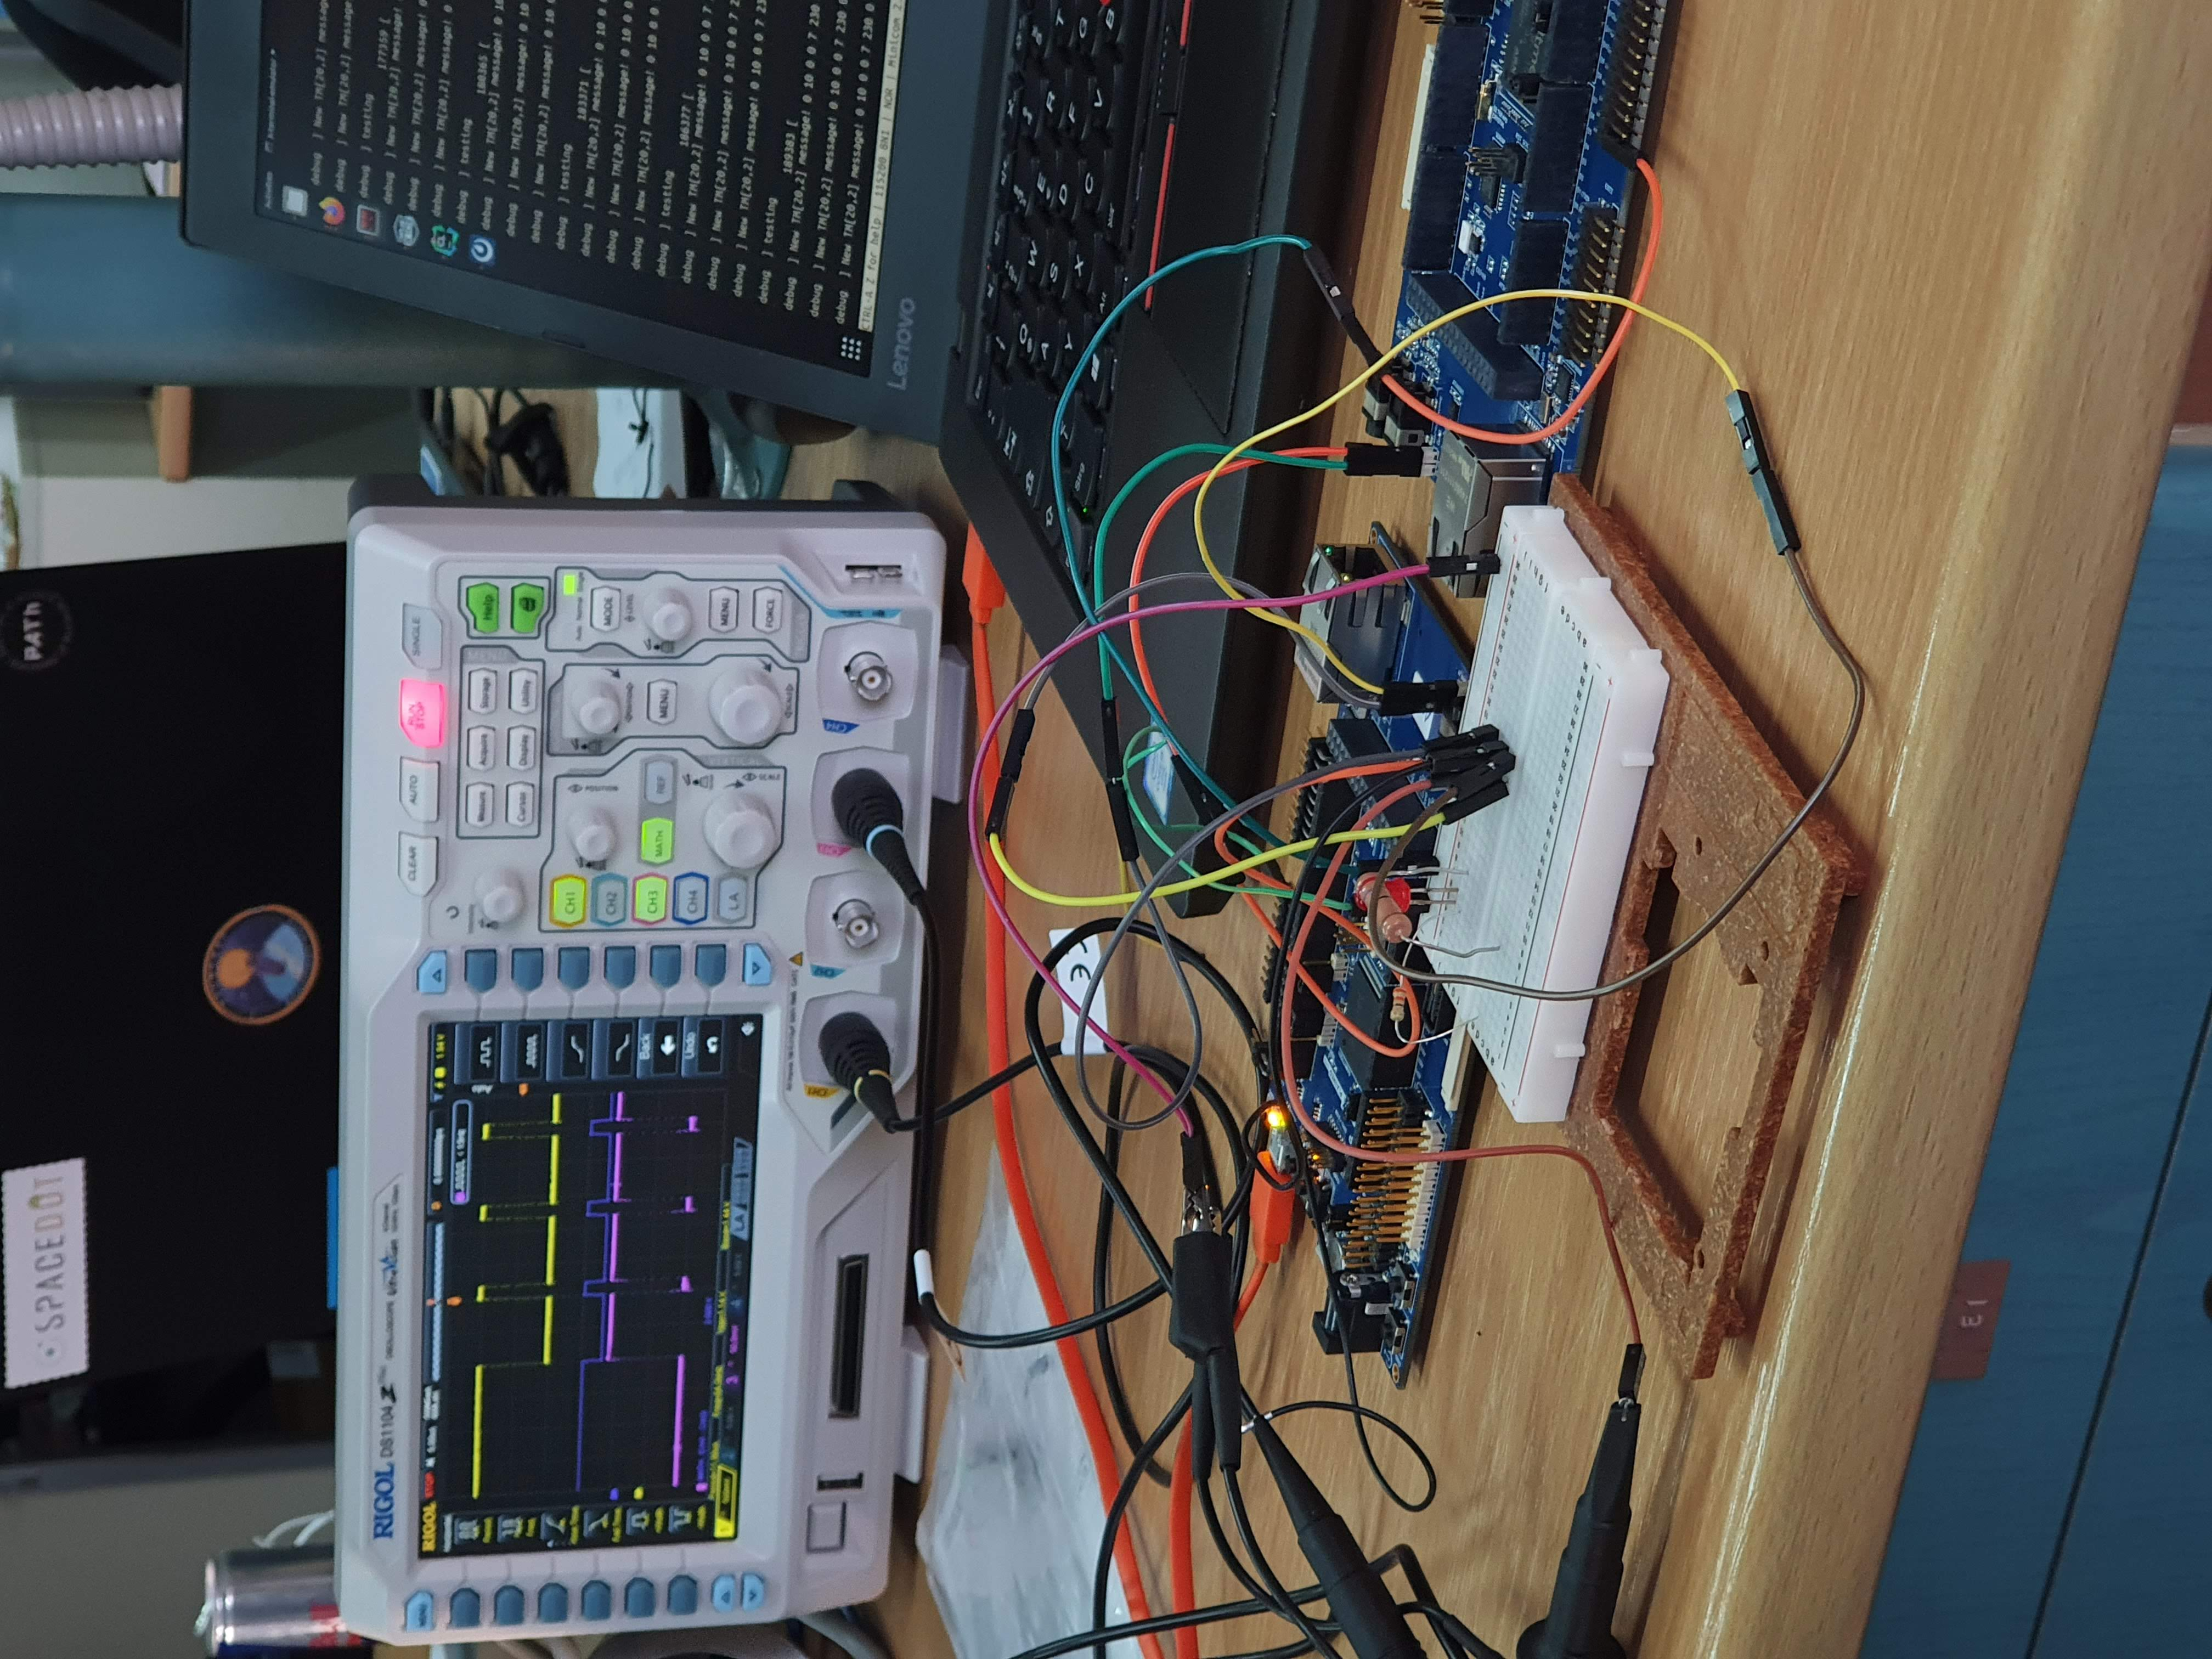
\includegraphics[angle=270,origin=c]{media/images/lab-wiring-scope.jpg}
\end{figure}

Το σύνολο της εργασίας μου έγινε υπό άδεια MIT, όπως λειτουργεί και το υπόλοιπο project του λογισμικού του δορυφόρου. Η άδεια αυτή επιτρέπει την οποιαδήποτε χρήση του λογισμικού, χωρίς άδεια από τον δημιουργό. Ο δημιουργός δεν παρέχει καμία εγγύηση, αλλά και καμία υποχρέωση καλής λειτουργίας του λογισμικού. 

Κατά τη διάρκεια της ανάπτυξης του λογισμικού η δουλειά μου καταγράφθηκε χρησιμοποιώντας το Git για Version Control στα αποθετήρια της ομάδας. Οι παρακάτω σύνδεσμοι οδηγούν στα σχετικά Merge Requests που έγιναν στο Gitlab της ομάδας. Εκεί φαίνεται ο χαρακτήρας της ομάδας, όσο αφορά το peer-review. Όλες οι αλλαγές που έγιναν στον κώδικα ελέγχθηκαν από τουλάχιστον δύο συμφοιτητές, πριν ενσωματωθούν στον κώδικα του δορυφόρου. 

\section{Περιορισμοί συστήματος}

Ο χαρακτήρας του συστήματος που αναπτύχθηκε είναι αυστηρά περιορισμένος από τους πόρους του μικροελεγκτή. Ο μικροελεγκτής που χρησιμοποιήθηκε έχει μόλις 384KB από στατική RAM διαθέσιμη για όλες τις λειτουργίες του κάθε υποσυστήματος. Περαιτέρω, για να επιτευχθούν στόχοι αξιοπιστίας η ομάδα αποφάσισε να απαγορεύσει την δυναμική εκχώρηση μνήμης στο λογισμικό του δορυφόρου. Οι δύο αυτοί περιορισμοί συνδράμουν στην δυσκολία της υλοποίησης, καθώς η ανάπτυξη γίνεται με την χρήση της γλώσσας C++, η οποία δεν παρέχει εύκολη υποστήριξη για την διαχείριση της μνήμης. Από την αρχή της ανάπτυξης του λογισμικού, η ομάδα επέλεξε να χρησιμοποιήσει την βιβλιοθήκη Embedded Template Library (ETL), η οποία προσφέρει συναρτήσεις ανάλογες της C++ Standard Library (STL). Η σημαντική διαφοροποίηση στις δύο βιβλιοθήκες είναι ότι η ETL δίνει τη δυνατότητα χρήσης αποκλειστικά \textbf{στατικά εκχωρημένης μνήμης}. Για να το επιτύχει αυτό, ο προγραμματιστής πρέπει να ορίσει το μέγιστο μέγεθος για όλους τους τύπους κοντέινερ. Για παράδειγμα, ένα μήνυμα πρέπει να έχει αυστηρά ορισμένο μέγεθος στον πίνακα των δεδομένων του, και μία ουρά πρέπει να έχει ορισμένο το μέγιστο μέγεθος της. Αυτός ο περιορισμός επιβάλλει την χρήση της μνήμης με πολύ προσεκτικό τρόπο, καθώς η χρήση μνήμης που δεν έχει αναλογιστεί μπορεί να οδηγήσει σε απρόβλεπτες συμπεριφορές του προγράμματος. Παρόλα αυτά, η ομάδα κατάφερε να υλοποιήσει ένα σύστημα που ικανοποιεί τις απαιτήσεις του δορυφόρου, χωρίς να θυσιάσει την αξιοπιστία του.

\section{Επίπεδα λογισμικού}

\begin{itemize}
	\item \textbf{Application Layer}: Το υψηλότερο επίπεδο κώδικα που θα χρησιμοποιηθεί στην αποστολή. Η χρήση των συναρτήσεων που έχουν υλοποιηθεί στο επίπεδο του Application Layer δεν απαιτεί καμία γνώση από το υπόλοιπο περιβάλλον υλοποίησης. Για παράδειγμα, η συνάρτηση \textbf{createRequestParametersMessage()} απαιτεί μόνο τον ορισμό του παραλήπτη, και του πίνακα με τα αναγνωριστικά παραμέτρων που ζητούνται. Η διαδικασία μετατροπής του μηνύματος στο πρωτόκολλο CAN-TP, η αποστολή και η λήψη από τον παραλήπτη γίνονται αυτόματα. Επίσης αυτόματη είναι η απάντηση του παραλήπτη με τη συνάρτηση \textbf{createSendParametersMessage()}, όπου αποστέλλονται οι παράμετροι που ζητήθηκαν στη μορφή που ορίστηκε από την ομάδα στο AcubeSAT specific πρωτόκολλο. Τέλος, το σύστημα διαβάζει το μήνυμα, ή τη σειρά μηνυμάτων, με τις παραμέτρους και ανανεώνει τις τιμές τους. Το επίπεδο αυτό είναι διαμορφωμένο με τρόπο ώστε να καλύπτει τις ανάγκες της αποστολής, όμως η υλοποίηση γενικεύεται αρκετά ώστε να μπορεί να αναπτυχθεί σε οποιαδήποτε αρχιτεκτονική χρειαστεί.
	\item \textbf{TP Protocol}: Το επίπεδο του TP Protocol αφορά το πακετάρισμα και την αποστολή μηνυμάτων μέσω του CAN. Είναι βασισμένο στο πρωτόκολλο ISO 15765, παραλείποντας τα μηνύματα που αφορούν τον έλεγχο ροής δεδομένων (Flow Control). Η χρήση του πρωτοκόλλου επιτρέπει την αποστολή μηνυμάτων με μέγεθος μεγαλύτερο από 64-byte, όπως ορίζεται από την επέκταση CAN-FD. Όταν είναι απαραίτητο, τα μηνύματα χωρίζονται και αναδιαμορφώνονται σε πακέτα των 64-byte, να απαιτέιται προεργασία στο μήνυμα από ανώτερα επίπεδα. Αυτή τη στιγμή το πρωτόκολλο CAN-TP υλοποιήθηκε με βασικό \textbf{Error Detection \& Handling}, λόγω περιορισμένων πόρων του συστήματος. Η ομάδα έχει σκοπό να αναπτύξει την υλοποίηση ώστε να καλύπτει συγκρούσεις και απώλεια δεδομένων με ευλάβεια, όταν έρθει η ώρα ανάπτυξης του συστήματος FDIR του δορυφόρου.
	\item \textbf{Driver}: Το χαμηλότερο επίπεδο κώδικα που σχετίζεται με τις ανάγκες της αποστολής. Το επίπεδο Driver περιέχεται στα αρχεία Driver.cpp και Driver.hpp, και οδηγεί το ενσωματωμένο περιφερειακό του μικροελεγκτή κατά τη διάρκεια της αρχικοποίησης αλλά και της αποστολής και λήψης δεδομένων. Στο επίπεδο αυτό ορίζονται συναρτήσεις που διαφέρουν ανά μικροελεγκτή, χάρη στη σύνδεση και το Application Programming Interface (API), που έχει οριστεί από τον κατασκευαστή. Οι συναρτήσεις αυτές περιλαμβάνουν την εξαγωγή δεδομένων από το περιφερειακό κατά τη διάρκεια ενός Interrupt Service Routine (ISR), η μετατροπή των δεδομένων του μηνύματος στην μορφή που χρησιμοποιεί ο κατασκευαστής, κ.α.
\end{itemize}

Είναι άξιο να σημειωθεί ότι το επίπεδο Driver είναι το μόνο επίπεδο που χρήζει τροποποίηση, όταν ο κώδικας μεταφέρεται σε διαφορετικό μοντέλο μικροελεγκτή. Για παράδειγμα, η ομάδα που συνδράμει στο project \textit{PeakSat} χρησιμοποιεί την υλοποίηση σε μικροελεγκτή της \textbf{STMicroelectronics}. Για την χρήση αυτή αντιγράφθηκαν οι επιλογές του περιφερειακού στο αντίστοιχο πρόγραμμα διαμόρφωσης, και τροποποιήθηκαν οι συναρτήσεις του Driver. Η επικοινωνία μεταξύ μικροελεγκτή STM και Atmel SAMV71 ήταν επιτυχής χωρίς καμία περαιτέρω αλλαγή. Χάρη στο υψηλό επίπεδο αφαίρεσης του Application Layer, είναι εύκολη και γρήγορη η ενσωμάτωση του κώδικα σε νέο περιβάλλον.

\section{Διεπαφή με τον κώδικα του περιφερειακού}
% talk about message IDs being shifted 11 bits to the left. Talk about 50MHz clock even though manufacturer recommends 20, 40, 80. Talk about needing a different fifo callback function for mcan0, mcan1, rxfifo0, rxfifo1

\section{Η διαδρομή ενός μηνύματος}

Τα περισσότερα μηνύματα που μεταφέρονται μέσω CAN είναι αυτοματοποιημένα και περιοδικά. Αφορούν κυρίως την μεταφορά παραμέτρων και τον έλεγχο της εύρυθυμης λειτουργίας του συστήματος. Για την περιοδική αποστολή των μηνυμάτων, μπορούμε να βασιστούμε στο λειτουργικό σύστημα που χρησιμοποιείται στον μικροελεγκτή, το FreeRTOS. Η υλοποίηση της λειτουργικότητας του CAN είναι στενά συνδεδεμένη με το λειτουργικό σύστημα, καθώς χρησιμοποιούονται συναρτήσεις αναμονής, ουρές και σημαιοφόροι που παρέχονται από αυτό. Με βάση τα παραπάνω, έχουν υλοποιηθεί οι διεργασίς που φαίνονται στο παρακάτω διάγραμμα.

% FSM Διαγραμμα με περιοδικη αποστολη μηνυματων, αποθηκευση μηνυματων στην ουρα

Όπως φαίνεται, βασιζόμαστε στην έννοια των FreeRTOS Task για γεγονότα που επιθυμούμε να εκτελούνται περιοδικά για την εκπλήρωση κάποιων προδιαγραφών, όπως
\begin{itemize}
	\item Την αποστολή παραμέτρων, για την εκπλήρωση του Data Housekeeping από το OBC.
	\item Τον συγχρονισμό του ακριβή χρόνου σε UTC, σε όλα τα υποσυστήματα.
	\item Την εκτέλεση διαδικασιών ανίχνευσης και διόρθωσης σφαλμάτων, μέσω περιοδικών μηνυμάτων \emph{παλμών}. Μέσα από αυτά το OBC ανιχνεύει υποσυστήματα τα οποία δεν αποκρίνονται και εκτελεί τις κατάλληλες ενέργειες για την επαναφορά τους. 
\end{itemize}

\section{Η μεταφορά μηνυμάτων ως πακέτα}

Από τον σχεδιασμό του πρωτοκόλλου του CAN Bus, ένα μήνυμα αποτελείται κατά μέγιστο από 8-byte στη κλασική έκδοση και 64-byte στην επέκταση CAN-FD. Σχεδόν όλοι οι δημιουργοί επεξεργαστών και μικροελεγκτών που αλληλεπιδρούν με το CAN χρησιμοποιούν πίνακες ορισμένων μεγέθων από μεταβλητές με τύπο uint8\_t στις γλώσσες C και C++. Οι μεταβλητές uint8\_t αναπαριστούν έναν ακέραιο αριθμό, μη-προσημασμένο, με μέγεθος 8-bit. Ο τύπος αυτός χρησιμοποιείται συχνά σε ενσωματωμένα συστήματα όταν η αναπαράσταση των δεδομένων είναι λιγότερο σημαντική από την μεταφορά ή την αποθήκευσή τους. Η επιλογή αυτή από τους κατασκευαστές οδήγησε σε δύο προβλήματα στην υλοποίηση της διεπαφής του πρωτοκόλλου της ομάδας με το περιφερειακό.

Αρχικά, τα μηνύματα που μεταφέρονται στο πρωτόκολλο CAN-TP πολύ συχνά μεταφέρουν μεταβηλτές με μέγεθος μεγαλύτερο από ένα uint8\_t. Η αρχική μου ιδέα στο παραπάνω θέμα, ήταν να χρησιμοποιήσω συναρτήσεις που χρησιμοποιούν πρότυπα (templates) και δέχονται μεταβλητές ανεξαρτήτου μεγέθους και τις εισάγουν κατάλληλα σε πίνακα που δέχεται μεταβλητές τύπου uint8\_t. Ένα παράδειγμα κώδικα σε C++ που υλοποιεί αυτή τη συνάρτηση φαίνεται παρακάτω. 

\inputminted{cpp}{code/stuffInVector.cpp}

Η λύση αυτή, παρόλο λειτουργική σε πρώτη ματιά, προσφέρει ελάχιστα από άποψη εργονομίας στον προγραμματιστή και ελέγχου και αναφοράς σφαλμάτων. Η υλοποίηση γεννά πολλές συζητήσεις όπως για παράδειγμα της συμπεριφοράς σε περίπτωση σφαλμάτων, ή της επιλογής Endianness των δεδομένων (εάν το πιο σημαντικό byte αποθηκεύεται στην προγενέστερη θέση μνήμης, χρησιμοποείται Big-Endian αναπαράσταση). Καθώς η διαδικασία υλοποίησης της εργασίας ήταν ήδη μεγάλη, αποφασίστηκε ότι δεν είναι εύλογο να παραχθεί κώδικας που ικανοποιεί τις απαιτήσεις της ομάδας.

Ευτυχώς, κατά της διάρκεια της ανάπτυξης του λογισμικού που υλοποιεί τα \href{https://gitlab.com/acubesat/obc/ecss-services}{ECSS Services}, δημιουργήθηκε η κλάση Message. Όπως αναφέρει η βιβλιογραφία των ECSS Services που αναπτύχθηκαν από την ομάδα, \textit{Το Message είναι ένα από τα δομικά στοιχεία της υλοποίησης των ECSS Services. Αυτή η κλάση αναπαριστά ένα μήνυμα τηλεμετρίας ή τηλε-εντολής. Το Message είναι η απλούστερη μονάδα πληροφοριών που μεταφέρεται μεταξύ του δορυφόρου και του σταθμού βάσης. Ένα Μήνυμα περιέχει τα δεδομένα του σε μορφή δυαδικής συμβολοσειράς, σε συνδυασμό με ορισμένες βασικές πληροφορίες της κεφαλίδας.} Στην υλοποίηση της κλάσης, η ομάδα επέλεξε το πεδίο δεδομένων του μηνύματος να αναπαριστάται από έναν πίνακα μεταβλητών τύπου uint8\_t, για τους ίδιους λόγους που αναφέρθηκαν παραπάνω. Η ομάδα επίσης υλοποίησε συναρτήσεις που γράφουν και διαβάζουν μεταβλητές οποιουδήποτε μεγέθους στο πεδίο δεδομένων της κλάσης Message. Για αυτή την ευκολία, αποφασίστηκε να χρησιμοποιηθεί η δυνατότητα κληρονομικότητας των κλάσεων στη C++ και να δημιουργηθεί η κλάση TPMessage από την Message.

Όπως αναφέρεται παραπάνω, η κλάση Message παρέχει μεθόδους που διευκολύνουν την ενσωμάτωση και την ανάγνωση μεταβλητών πολλών τύπων, παρά την εσωτερική δομή της κλάσης. Στο παράδειγμα παρακάτω φαίνεται ο τρόπος με τον οποίο αποθηκεύουμε και διαβάζουμε μεταβλητές στη κλάση.
\inputminted{cpp}{code/ecss-message-usage.cpp}

Η κλάση TPMessage επίσης προσφέρει συναρτήσεις που κωδικοποιούν και αποκωδικοποιούν το πεδίο ID ενός CAN-TP μηνύματος και τα κατάλληλα πεδία που αποθηκεύουν αυτή την πληροφορία. Ως παράγωγη κλάση της Message, η κλάση TPMessage περιέχει όλα τα πεδία της Message. Ορισμένα από αυτά αναφέρονται στον τύπο της υπηρεσίας που αναφέρεται το Message και εάν αυτό είναι τηλεμετρία ή τηλε-εντολή. Εφ'όσον αυτά τα πεδία δεν έχουν κάποια σημασία στο σκοπό ενός TPMessage, έχει σημειωθεί ότι η ομάδα πρέπει να τροποποιήσει κατάλληλα στο μέλλον την δομή ενός Message ώστε να αποφευχθούν είτε μελλοντικά λάθη κατανόησης, είτε η σπατάλη μνήμης από τους περιορισμένους πόρους του δορυφόρου. 

Όπως αναφέρθηκε προηγουμένως, ο μικροελεγκτής που χρησιμοποιείται υποστηρίζει την επέκταση του πρωτοκόλλου CAN-FD. Χάρη σε αυτή την επέκταση, έχουμε τη δυνατότητα να στείλουμε μηνύματα μεγαλύτερα των 8-byte που υποστηρίζονται από το κλασικό CAN. Φυσικά, με την προϋπόθεση ότι όλοι οι κόμβοι του δικτύου υποστηρίζουν την επέκταση του πρωτοκόλλου, την οποία η ομάδα εξασφάλισε να καλύπτουν όλοι οι κόμβοι που επικοινωνούν στο δίαυλο.

Για την κάλυψη των αναγκών της αποστολής, είναι απαραίτητη η ανάπτυξη ενός πρωτοκόλλου για την πακετοποίηση και την μεταφορά μηνυμάτων των οποίων το μέγεθος ξεπερνά τα 64-byte. Με βάση το πρωτόκολλο CAN-TP, υλοποιήθηκε ένας μηχανισμός που δέχεται μηνύματα ανεξαρτήτου μεγέθους (με πραγματικό όριο τα 1024-byte λόγω περιορισμών μνήμης), και τα χωρίζει σε πακέτα των 64-byte όταν αυτό κρίνεται απαραίτητο. Για την μεταφορά αυτών των μηνυμάτων, το TP μήνυμα ενθυλακώνεται σε ένα ή περισσότερα μηνύματα CAN (ή αλλιώς Frames), τα οποία μεταφέρονται στο δίαυλο. Το παρακάτω διάγραμμα περιγράφει την διαδικασία αυτή. 

% excalidraw diagram of encapsulation of a acubesat tp message with first byte

Όπως φαίνεται στο σχήμα, το πρώτο byte ενός Frame παρέχει πληροφορίες για τη θέση του ίδιου σε ένα μεγαλύτερο σύνολο μηνυμάτων. Συγκεκριμένα, υπάρχουν τέσσερις τύποι μηνυμάτων στο πρωτόκολλο CAN-TP, τα οποία περιγράφονται στον παρακάτω πίνακα.

\begin{itemize}
	\item \textbf{Single Frame}: Το CAN-TP μήνυμα περιέχεται σε ένα μόνο Frame. Το πρώτο byte περιέχει τον συνδυασμό του αναγνωριστικού ενός Single Frame μηνύματος και το μέγεθος των δεδομένων του. Τα επόμενα 63 bytes περιέχουν τα δεδομένα του.
	\item \textbf{First Frame}: Το CAN-TP μήνυμα ξεκινά με αυτό το Frame. Η διαφοροποίηση του First Frame από τα επόμενα είναι σημαντική καθώς με την λήψη του First Frame εκκαθαρίζεται η ουρά εισερχόμενων μηνυμάτων τύπου CAN-TP. Η εκκαθάριση είναι απαραίτητη καθώς τα μηνύματα συγχωνεύονται σε ένα αντικείμενο τύπου TPMessage, συνενώνοντας τα ενθυλακωμένα δεδομένα κάθε μηνύματος με βάση τη θέση τους στην ουρά. Εάν στην ουρά υπάρχουν ήδη μηνύματα που δεν σχετίζονται με το εισερχόμενο, αυτό θα οδηγήσει σε απροσδιόριστη συμπεριφορά. Παραπάνω ανάλυση του τομέα με πιθανές λύσεις δίνεται σε επόμενη ενότητα. Το πρώτο byte περιέχει τον συνδυασμό του αναγνωριστικού ενός First Frame και τον αριθμό των μηνμάτων που απαρτίζουν ολόκληρο το CAN-TP μήνυμα. Τα υπόλοιπα 63 bytes περιέχουν τα δεδομένα του.
	\item \textbf{Consecutive Frame}: Το CAN-TP μήνυμα περιέχεται σε ένα Frame, και είναι συνέχεια του First Frame. Το πρώτο byte περιέχει τον συνδυασμό του αναγνωριστικού ενός Consecutive Frame και την θέση του στην ουρά των μηνυμάτων. Τα υπόλοιπα 63 bytes περιέχουν τα δεδομένα του.
	\item \textbf{Final Frame}: Το CAN-TP μήνυμα τελειώνει με αυτό το Frame. Παρόλο που είναι δυνατό να υπολογίσουμε αν το CAN-TP μήνυμα έχει ληφθεί ολόκληρο με βάση τον αριθμό των Consecutive Frame που έχουμε δεχτεί, η χρήση του Final Frame διευκολύνει την αναγνωσιμότητα του κώδικα και προσφέρει ταχύτητα. Το επίπεδο του Driver εκτελεί την επεξεργασία της ουράς των μηνυμάτων μόλις δεχτεί ένα Frame με αυτό το byte, χωρίς να χρειαστεί η αποθήκευση και ανάγνωση του αριθμού μηνυμάτων στην ουρά. 
\end{itemize}

Η παραπάνω διαδικασία έχει φανεί αξιόπιστη σε δοκιμές με τρείς κόμβους στο δίκτυο, παρά την απουσία μηχανισμών εντοπισμού και αποκατάστασης σφαλμάτων. Το παραπάνω φαινόμενο είναι δυνατό λόγω της αυτόματης προτεραιότητας στον δίαυλο, που εξασφαλίζεται από το πρωτόκολλο. Επειδή η τοποθέτηση μηνυμάτων στην θυρίδα αποστολής σε επίπεδο κώδικα γίνεται σε βρόγχο με ελάχιστη υπολογιστική πολυπλοκότητα, μπορούμε να θεωρήσουμε ότι γίνεται αστραπιαία. Στη συνέχεια, ο συνδυασμός του περιφερειακού με τον transceiver του κόμβου θα αποστείλει τα μηνύματα στο δίαυλο σειριακά. Το αναγνωριστικό ενός CAN-TP μηνύματος, όπως ορίστηκε από την ομάδα, περιέχει το αναγνωριστικό του αποστολέα στα περισσότερο-σημαντικά bit. Χάρη στο παραπάνω, η προτεραιότητα που ορίστηκε για τα μη-CAN-TP μηνύματα ισχύει με τον ίδιο τρόπο. Ως αποτέλεσμα, 

\section{Λειτουργία του Gatekeeper}

% ref freertos manual gatekeeper task
Σε περίπλοκα ενσωματωμένα συστήματα που χρησιμοποιούν το FreeRTOS, συνιστάται η υλοποίηση των Gatekeeper Task. Κάθε περιφεριακό απαιτεί το δικό του Gatekeeper Task. Ο σκοπός του Task είναι η διασφάλιση των συναλλαγών με το περιφεριακό, και αυτό επιτυγχάνεται με την αποκλειστική πρόσβαση του Task στο περιφερειακό. Η ομάδα έχει ακολουθήσει αυτή την πρακτική σε όλα τα περιφερειακά που χρησιμοποιούνται στο λογισμικό του δορυφόρου έως σήμερα, συμπεριλαμβανομένου του περιφερειακού για το CAN. Ως εκ τούτου, κάθε διεργασία που απαιτεί την αποστολή δεδομένων μέσω CAN χρησιμοποιεί τις συναρτήσεις του CANGatekeperTask. Η υλοποίηση χρησιμοποιεί δύο στατικά εκχωρημένες ουρές του FreeRTOS. Οι ουρές κρατούν αντικείμενα τύπου Frame, τα οποία διατηρούν πληροφορίες για το αναγνωριστικό (ID) και τα δεδομένα ενός μηνύματος. Όπως θεωρείται αυτονόητο, η φύση της ουράς είναι First-in-First-out (FIFO). Μία μέθοδος για παράκαμψη της ουράς σε περίπτωση σημαντικών μηνυμάτων συζητήθηκε, όμως απορρίφθηκε λόγω της πολυπλοκότητας που θα προσέφερε στον κώδικα. Η συμπεριφορά στην περίπτωση που η ουρά είναι ήδη γεμάτη οδηγεί στην απώλεια εξερχομένων μηνυμάτων, κάτι που δεν θεωρείται αποδεκτό στο πλαίσιο του πειράματος.

\par Η χρήση ουρών από το FreeRTOS κατέληξε εξαιρετικά βολική λόγω της ενσωμάτωσης της στη διεπαφή του IDE που χρησιμοποείται, του CLion. Χρησιμοποιώντας δύο εντολές στον κώδικα, το CLion δύναται να διαβάσει τα περιεχόμενα της ουράς ανά πάσα στιγμή και να τα εμφανίσει στο μενού αποσφαλμάτωσης κώδικα. Η λειτουργία αυτή φάνηκε ιδιαίτερα χρήσιμη κατά τη διάρκεια της ανάπτυξης του λογισμικού του δορυφόρου και κατέληξε να χρησιμοποείται σε όλες τις αντίστοιχες ουρές Gatekeeper του δορυφόρου.

% screenshot of CLion debug using CAN Queue View

\par Το CANGatekeperTask είναι εξίσου υπεύθυνο για την διαχείριση των ρυθμίσεων του περιφερειακού σε χαμηλότερο επίπεδο. Με κάθε εκτέλεση, έχει δύο αρμοδιότητες. Αρχικά, ρυθμίζει τις εισόδους CAN\_SILENT των transceivers. Οι CAN Transceivers έχουν τη δυνατότητα να τεθούν σε \textit{αθόρυβη} λειτουργία, στην οποία απαγορεύεται να στέλνουν μηνύματα στο δίαυλο. Σε αυτή τη λειτουργία επιτρέπεται μόνο να απαντούν σε μηνύματα με την αναγνώριση μηνυμάτων (ACK), όταν αυτό κρίνεται απαραίτητο. Προς το παρόν, όλοι οι κόμβοι του δικτύου απενεργοποιούν τη λειτουργία, καθώς όλα τα υποσυστήματα συμμετέχουν στο δίαυλο. Μελλοντικά, κατά την ανάπτυξη του FlatSat, η ομάδα εξετάζει την συμπερίληψη μίας εξωτερικής πλακέτας για την αναγνώριση σφαλμάτων στο δίαυλο. Για να ελαχιστοποιηθεί η επιρροή της πλακέτας στο σύστημα, αυτή θα τεθεί στην αθόρυβη λειτουργία της με την παραπάνω ρύθμιση. Η δεύτερη αρμοδιότητα του CANGatekeperTask είναι να αρχικοποιεί τα κυκλώματα Latchup Current Limiter (LCL) που χρησιμοποιούνται στο OBC/ADCS Board. Τα κυκλώματα αυτά .

\par Περιοδικά, το Task εκτελεί μία διαδικασία εντοπισμού σφαλμάτων, υπολογίζοντας τον χρόνο από την τελευταία επιτυχή αποστολή δεδομένων. Εάν ο χρόνος αυτός υπερβεί τα 8 δευτερόλεπτα τα LCL επαναφέρονται, μαζί με το εσωτερικό περιφερειακό του επεξεργαστή. Έπειτα, τα μηνύματα που αναμένουν αποστολή στην ουρά εξερχομένων αποστέλλονται. Ο χρόνος επιλέχθηκε πειραματικά. Καθώς ακόμα δεν έχει οριστικοποιηθεί το περιεχόμενο και η περίοδος των περιοδικών μηνυμάτων, η επιλογή αυτή δεν είναι τελική.

\par Τέλος, το CANGatekeeperTask εκτελεί και το βασικό του ρόλο, να επιμελείται την πρόσβαση στο περιφερειακό του CAN. Οποιαδήποτε άλλη διεργασία που σκοπεύει να στείλει μηνύματα στο δίαυλο χρησιμοποιεί τις ρουτίνες του CANGatekeperTask, προσθέτοντας τα μηνύματα προς αποστολή στην ουρά εξερχομένων. Με τη σειρά του, το CANGatekeeperTask στέλνει αυτά τα μηνύματα όταν έρθει η σειρά του με βάση την προτεραιότητα που έχει οριστεί στο τεμαχισμό χρόνου από το λειτουργικό σύστημα (FreeRTOS).

\section{Διαφοροποίηση στα CAN-TP και non-CAN-TP μηνύματα}

Η διαφοροποίηση μεταξύ των μηνυμάτων μορφής CAN-TP και μή γίνεται με χρήση του αναγνωριστικού τους. Μία σημαντική λεπτομέρεια για την απόδοση της υλοποίησης σε χρόνο επεξεργαστή και χρήση μνήμης είναι αυτή η διαφοροποίηση να γίνεται στο χαμηλότερο δυνατό επίπεδο. Σχεδόν κάθε περιφειακό CAN σε μικροελεγκτή έχει την δυνατότητα ορισμού κάποιων \textit{φίλτρων}, που καθοδηγούν τα μηνύματα στη σωστή ουρά FIFO ανάλογα με το αναγνωριστικό τους. Όπως αναφέρθηκε προηγουμένως, τα μηνύματα που αφορούν διαδικασίες CAN-TP χρησιμοποιούν ειδική μορφή στο αναγνωριστικό τους. Σε επίπεδο bit το αναγνωριστικό ξεκινά με τον συνδυασμό $0b01110000000$, και τα υπόλοιπα δεδομένα προστίθενται με διαδικασίες bitwise-OR στις αντίστοιχες θέσεις. Το πλεονέκτημα αυτής της υλοποίησης είναι ότι μπορούμε να ξεχωρίσουμε τα μηνύματα CAN-TP, αφού βρούμε τα άνω και κάτω όρια της τιμής του ID. Στην περίπτωση που έχουμε παντού άσσους θα έχουμε:

\begin{equation}
0b0111`111`111`1 = 0x3FF
\end{equation}

και στην περίπτωση που έχουμε παντού μηδενικά θα έχουμε:
\begin{equation}
0b0111`000`000`0 = 0x300
\end{equation}

Με αυτή τη πληροφορία, μπορούμε πλέον να ορίσουμε το φίλτρο που θα οδηγήσει τα μηνύματα που δεν αφορούν CAN-TP δεδομένα. Ο μικροελεγκτής ATSAMV71Q21B προσφέρει τρία διαθέσιμα \textit{μονοπάτια} για τα εισερχόμενα μηνύματα. Δύο από αυτά είναι ουρές τύπου FIFO με ονόματα RX-FIFO-0 και RX-FIFO-1. Η τρίτη ουρά ονομάζεται Message Buffer και χρησιμοποιεί μία θυρίδα για κάθε ορισμένο ID μηνύματος. Στην υλοποίηση χρησιμοποιούνται αποκλειστικά οι δύο ουρές τύπου FIFO. Στην ουρά με όνομα RX-FIFO-0 δρομολογούνται τα μηνύματα τύπου CAN-TP και στην ουρά με όνομα RX-FIFO-1 δρομολογούνται τα υπόλοιπα.

Με τα μηνύματα αυτόματα χωρισμένα, είναι εύκολο πλέον να ορίσουμε τις ρουτίνες που εκτελούνται στο μηχανισμό interrupt για την λήψη μηνυμάτων CAN. Δημιουργήθηκαν δύο συναρτήσεις οι οποίες αρχικά λαμβάνουν τα μηνύματα από την εσωτερική RAM που χρησιμοποιεί το περιφερειακό. Η μία συνάρτηση χρησιμοποιείται για τα TP μηνύματα και πρώτο αναλύει τον τύπο του μηνύματος. Εάν αυτό αποτελεί μέρος μεγαλύτερου μηνύματος προστίθεται στην ουρά εισερχόμενων μηνυμάτων που αναφέρθηκε παραπάνω. Εάν είναι αυτόνομο ή εάν είναι το τέλος ενός CAN-TP μηνύματος πολλαπλών κομματιών, εκτελείται η διαδικασία επανένωσης και ανάγνωσης του μηνύματος.

Στην περίπτωση που το εισερχόμενο μήνυμα δεν είναι τύπου CAN-TP, όπως δηλαδή ένα μήνυμα παλμού ή εναλλαγής ενεργού CAN Bus, αυτό διαβάζεται κατ'ευθείαν για εξοικονόμηση χρόνου επεξεργαστή μέσα στο Interrupt Service Routine (ISR). 

\section{Αυτοματισμοί}


\section{Χρήση δύο ανεξάρτητων διαύλων}
% parameter for changing the active bus. each subsystem can send data on either bus and nothing wrong will happen. you can disable receiving on bus 1 if you're using 2, discuss advantages and disadvantages of that. talk about main/redundant naming scheme. talk about bus switchover messages
\chapter{Χρήση της υλοποίησης}
\section{Χρήση στο Environmental Testing Campaign του OBC/ADCS Board}
	\subsection{Σκοπός environmental testing}
	Όπως αναφέρθηκε προηγουμένως, ένα σημαντικό επίτευγμα της ομάδας και πιο συγκεκριμένα, του υποσυστήματος 
	του OBC, είναι ο σχεδιασμός και η ανάπτυξη της πλακέτας OBC/ADCS Board.
% insert 3d render of OBC/ADCS Board

	\begin{figure}[h]
		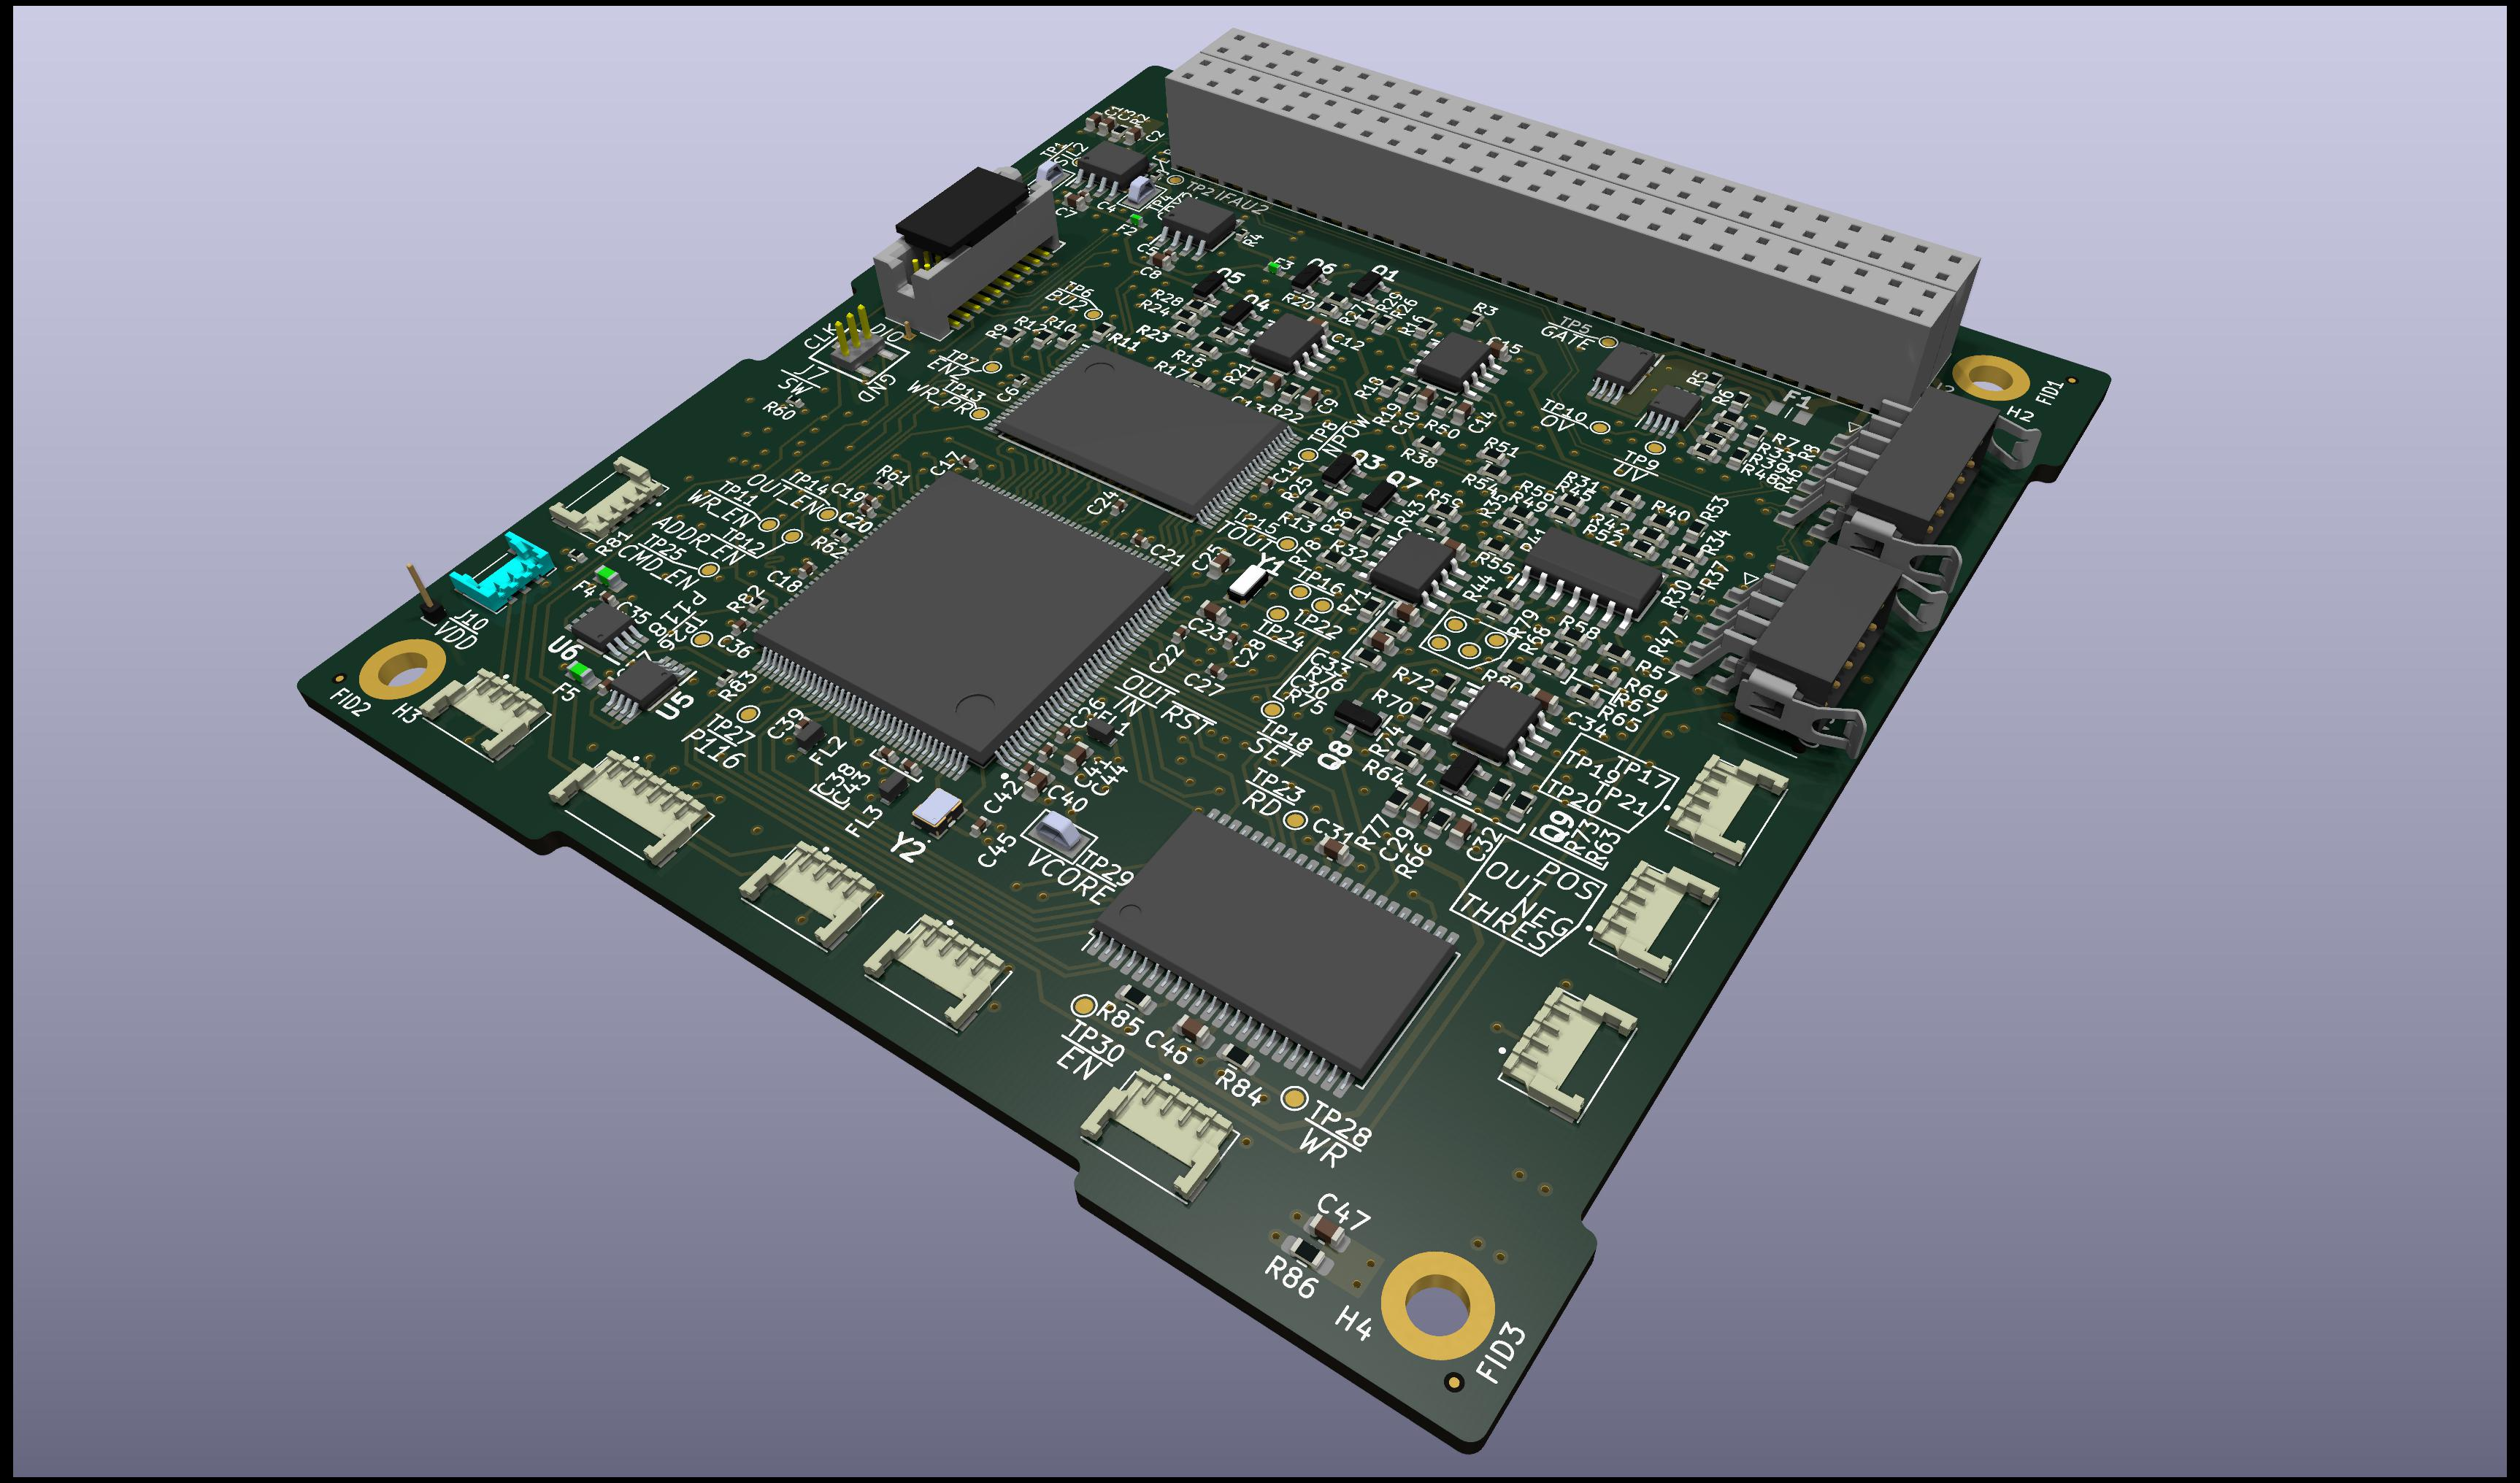
\includegraphics{media/images/obc-adcs-board.jpg}
	\end{figure}

	\par Όπως ορίζεται από τις οδηγίες του Ευρωπαϊκού Οργανισμού Διαστήματος (ESA), όλα τα στοιχεία του δορυφόρου να περάσουν μία σειρά από δοκιμές που θα επιβεβαιώσουν την ορθή λειτουργία της σε περιβάλλον διαστήματος. Οι δοκιμές αυτές ονομάζονται Environmental Testing και περιλαμβάνονται στην διαδικασία κατασκευής και επιβεβαίωσης του νανοδορυφόρου στο πρόγραμμα \textit{Fly Your Satellite!}.

	% ref vibe_tstp
	Καθώς το OBC/ADCS Board είναι κατασκευασμένο εξ'ολοκλήρου από την ομάδα, η ομάδα κλήθηκε να εκτελέσει αυτές τις δοκιμές στη πλακέτα, προτού αυτή μπορεί να θεωρηθεί ότι αρμόζει σε διαστημική αποστολή. Αρχικά, η πλακέτα τοποθετείται απενεργοποιημένη σε μία μεταλλική πλάκα, όπου διεξάγεται το Vibration Test. Κατά τη διάρκεια της δοκιμής, η πλάκα δονείται με τυχαίο και έντονο τρόπο, προσομοιώνοντας τις δονήσεις και τις δυνάμεις που θα υποστεί η πλακέτα κατά τη διάρκεια της εκτόξευσης. Ο σκοπός της δοκιμής αυτής είναι να εξετάσει την αντοχή της πλακέτας, των ολοκληρωμένων κυκλωμάτων πάνω σε αυτή, αλλά και την ποιότητα της εργασίας που έγινε για την συγκόλλησή της. Στην περίπτωση του OBC/ADCS Board, η δοκιμή αυτή έγινε με επιτυχία, καθώς η πλακέτα δεν υπέστη καμία ζημιά και η λειτουργία της δεν επηρεάστηκε.

	% ref tvac_tstp
	Η δεύτερη δοκιμή που διεξάγεται με βάση τις προδιαγραφές της ESA είναι το Thermal Vacuum Test. Κατά τη διάρκεια αυτού του Test, η πλακέτα τοποθετείται στο εσωτερικό του Thermal Vacuum Chamber (TVAC). Ο θάλαμος TVAC μεταφέρεται σε πίεση $10^{-5} hPa$, πίεση που είναι αρκετά χαμηλή ώστε να προσομοιώσει την πίεση στο διάστημα, χωρίς όμως να αποτελέσει τροχοπέδη για την διεξαγωγή του πειράματος σε εύλογο χρονικό διάστημα. Η διεξαγωγή πειραμάτων σε χαμηλή πίεση προσομοιώνει τη λειτουργία στο διάστημα και εντοπίζει σφάλματα στην διαδικασία παραγωγής της πλακέτας, όπως Solder Voids. Κατά τη διάρκεια της συγκόλλησης, μπορούν να δημιουργηθούν τρύπες γεμάτες με αέρα μέσα στις ενώσεις των μετάλλων. Όταν η πλακέτα τοποθετηθεί σε κενό αέρος, ο παγιδευμένος αέρας ασκεί δύναμη στις ενώσεις των μετάλλων, όσο προσπαθεί να δραπετεύσει. Αυτή η δύναμη μπορεί να προκαλέσει σπασίματα στις ενώσεις, προκαλώντας σοβαρή ζημιά στην πλακέτα. Στην περίπτωση του OBC/ADCS Board, η δοκιμή αυτή έγινε με επιτυχία, καθώς η πλακέτα δεν υπέστη καμία ζημιά και η λειτουργία της δεν επηρεάστηκε.

	\par Το δεύτερο κομμάτι του Thermal Vacuum Test αφορά την μελέτη της συμπεριφοράς του συστήματος σε θερμοκρασίες ανάλογες με αυτές που θα συναντήσει κατά τη λειτουργία του σε τροχιά. Όσο η πλακέτα βρίσκεται στο θάλαμο σε κενό αέρος, ο χειριστής μεταβάλλει την θερμοκρασία του θαλάμου έως ότου η πλακέτα να φτάσει στην επιθυμητή θερμοκρασία. Στην περίπτωση του OBC/ADCS Board, αυτό το εύρος θερμοκρασιών είναι $[-31,+64] ^o C$. Όπως αναφέρεται παρακάτω, το σύστημα εμφάνισε σφάλμαατα κατά τη διάρκεια της μεταβολής θερμοκρασίας.

	\subsection{Ανάλυση υλικού}
	% eqm kicad screenshots of transceivers
	Το OBC/ADCS Board τοποθετεί το OBC και το ADCS σε αντίθετες πλευρές, με κάθε υποσύστημα να διαθέτει δύο CAN transceivers. Η επικοινωνία μέσω του CAN κατά τη διάρκεια της εκστρατείας εξασφαλίζει τη μεταφορά παραμέτρων από το ADCS στο OBC, επιτρέποντας στο OBC να εκτελέσει λειτουργίες Data Housekeeping και Logging. Οι παράμετροι που μεταφέρονται περιλαμβάνουν μετρήσεις από τους αισθητήρες θερμοκρασίας, το μαγνητόμετρο και τα γυροσκόπια. Καθ' όλη τη διάρκεια της εκστρατείας, θα διασφαλίζεται η ομαλή λειτουργία της διαδρομής εκτέλεσης των τηλε-εντολών από τον σταθμό βάσης, όπου ο ρόλος του υποσυστήματος τηλεπικοινωνιών.

	Οι δίαυλοι του CAN Bus συνυπάρχουν στον κοννέκτορα PC/104, ο οποίος χρησιμοποιείται ως ένα από τα μέσα τροφοδοσίας των υποσυστημάτων στο νανοδορυφόρο. Παρακάτω φαίνεται ο κοννέκτορας PC/104 και οι δύο δίαυλοι CAN Bus, στο σχηματικό του OBC/ADCS Board που σχεδιάστηκε από την ομάδα. Η σύνδεση των διαύλων μέσα από τον κοννέκτορα PC/104 χρησιμεύει μόνο κατά τη διάρκεια της διαδικασίας κατασκευής και ελέγχου λειτουργίας του νανοδορυφόρου σε επίπεδο υποσυστήματος/συστήματος. Κατά τη διάρκεια της αποστολής, οι δίαυλοι χρησιμοποιούν διαφορετικούς κοννέκτορες που απέχουν $1,7cm$ μεταξύ τους. Ο σκοπός αυτής της επιλογής είναι η αποφυγή της πιθανότητας η βλάβη ενός κοννέκτορα να επηρεάσει και τους δύο διαύλους. 
	
	\subsection{Χρήση εξωτερικής πλακέτας για μεταφορά Log μηνυμάτων}
	Όσο η πλακέτα βρίσκεται στον θάλαμο κενού-θερμότητας (Thermal-Vacuum Chamber), το OBC/ADCS Board συνδέεται με τον υποστηρικτικό εξοπλισμό με βοήθεια ενός καλωδίου που παρέχει τροφοδοσία και μεταφέρει τα απαραίτητα σήματα UART, CAN και SWD για την προετιμασία της πλακέτας και τη διαδικασία που αναφέρθηκε παραπάνω.
	
	Στο πλαίσιο του σχεδιασμού του υποστηρικτικού εξοπλισμού για την εκστρατεία του OBC/ADCS Environmental Testing, η ομάδα αποφάσισε να χρησιμοποιήσει μια εξωτερική πλακέτα, την SAMV71 Xplained Board. Αυτή η πλακέτα θα συνδέεται μέσω CAN με την πλακέτα OBC/ADCS. 
	% insert diagram of connection and photo from cleanroom

	Η πλακέτα SAMV71 Xplained Board, που αποτελεί μέρος του υποστηρικτικού εξοπλισμού για την εκστρατεία OBC/ADCS, έχει ως σκοπό την προσομοίωση του υποσυστήματος τηλεπικοινωνιών. Αυτό επιτυγχάνεται μέσω της μετατροπής σειριακών δεδομένων από το σταθμό βάσης σε μορφή μηνυμάτων CAN και αντίστροφα. Η χρήση αυτής της πλακέτας αποβλέπει στην ελάφρυνση του φόρτου από το μικροελεγκτή του OBC και στην καλύτερη προσομοίωση των αρμοδιοτήτων του κατά τη διάρκεια της αποστολής.

	Για τη σύνδεση στο δίαυλο, δημιουργήθηκε το Shield PCB. Η πλακέτα στεγάζει τους απαραίτητους κονέκτορες και έναν επιπλέον transceiver, καθώς η πλακέτα SAMV71 Xplained περιέχει μόνο ένα. Ο δεύτερος transceiver χρησιμοποιείται για την επικοινωνία στο Redundant Bus.
	
	Από τις πρώτες δοκιμές αντιλήφθηκε ότι η λειτουργία δεν ήταν αξιόπιστη και η διάγνωση ήταν ότι οφείλεται στη χρήση διαφορετικών transceivers, των ATA6561 της Microchip σε αντίθεση με τους TCAN337 της Texas Instruments. Παρόλο που και τα δύο μοντέλα ακολουθούν τo στάνταρ ISO11898-1 για το CAN-FD, η επικοινωνία χανόταν εύκολα. Δημιουργήθηκε δεύτερη έκδοση που περιέχει τους κατάλληλους transceivers, αλλά και πάλι ο “συγχρονισμός” ήταν ασταθής και έπρεπε να γίνουν reset οι μικρoελεγκτές ταυτόχρονα. Παρά τη χρήση των αντιστάσεων τερματισμού που συνιστώνται από τον κατασκευαστή των TCAN337 CAN Transceivers, τα σφάλματα δεν ελαττώθηκαν. Η ομάδα καθήλωσε ότι τo μήκoς της σύνδεσης είvαι υπερβολικά μεγάλo στα 4m. Για να μειωθεί η πολυπλοκότητα του εξοπλισμού υποστήριξης, η ομάδα αναθεώρησε το πλάνο και χρησιμοποίησε τη σύνδεση UART του OBC για την επικοινωνία από και προς τον υπολογιστή.
	\subsection{Λειτουργία αυτόματης επαναφοράς μετά από σφάλματα}
	Μετά από την απόκτηση εμπειρίας στην επαναφορά μετά από παρατεταμένα σφάλματα στο CAN, δημιουργήθηκε μια πρώιμη μορφή FDIR για την επικοινωνία στο δίαυλο. Αναλύοντας την περιοδικότητα των μηνυμάτων, προγραμματίστηκε αυτόματη επαναφορά του transceiver και του ενσωματωμένου block περιφερειακού σε περίπτωση που δεν έχει επιτευχθεί επιτυχής αποστολή στα τελευταία X δευτερόλεπτα. Η λειτουργία αυτή φάνηκε χρήσιμη σε περιπτώσεις όπου ένα από τα δύο υποσυστήματα έκανε επανεκκίνηση, ενώ το άλλο βρισκόταν στη διαδικασία αποστολής TP μηνυμάτων. Η ουρά εξερχόμενων μηνυμάτων στο περιφερειακό του αποστολέα γέμιζε και η αποστολή μηνυμάτων σταμάτησε.

	Με την ενσωμάτωση της παραπάνω διαδικασίας διόρθωσης σφαλμάτων, ο μικροελεγκτής κατάφερε να επαναφέρει τη λειτουργία με υψηλή αξιοπιστία. Αυτό επέτρεψε στο σύστημα να συνεχίσει να λειτουργεί αδιάλειπτα για τη διάρκεια του χαρακτηρισμού του γυροσκοπίου του ADCS, που διήρκησε μία ώρα.

	\subsection{Μεταφορά παραμέτρων και μηνυμάτων τηλε-εντολών/τηλεμετρίας}
	Η τροποποίηση του λογισμικού για να καλύψει τις ανάγκες του Environmental Testing Campaign ήταν ευκολότερη χάρη στο application layer. Δημιουργήθηκε ένα περιοδικό task στο FreeRTOS, το οποίο καλούσε μία μόνο συνάρτηση αποστολής παραμέτρων στο ADCS. Η λήψη και η αποθήκευση των παραμέτρων από το OBC γίνονταν αυτόματα με βάση τον κώδικα που είχε ήδη γραφτεί. Η μεταφορά των τηλε-εντολών υλοποιήθηκε μέσω της δημιουργίας ενός ακόμη "service" στο αποθετήριο των ECSS Services. Αυτό το service μετέδιδε όλες τις τηλε-εντολές στο ανάλογο υποσύστημα, με βάση τo ECSS Application Process ID.

	Τέλος, η μεταφορά των log μηνυμάτων γίνεται με μία μόνο κλήση συνάρτησης του Application Layer, όπου ο χρήστης αντικαθιστά τη χρήση του περιφερειακού UART με τη συνάρτηση CAN::sendLogMessage.
	\subsection{Διακοπή λειτουργίας σε υψηλή θερμοκρασία}
	Λόγω παγκοσμίων προβλημάτων στην αλυσίδα εφοδιασμού κατά την παραγωγή της πλακέτας του OBC/ADCS, χρησιμοποιήθηκαν διαφορετικά TCXO (Temperature Compensated Crystal Oscillator - ένας τύπος κρυστάλλου που χρησιμοποιείται για τη δημιουργία σταθερής συχνότητας σε ηλεκτρονικές συσκευές, όπως τα ρολόγια) στα OBC και ADCS. Τα ρολόγια είχαν τις ίδιες μηχανικές ιδιότητες, ωστόσο, λειτουργούσαν στα 16MHz αντί για 12MHz. Στη θέση τους, χρησιμοποιήσαμε το ενσωματωμένο κύκλωμα RC του μικροελεγκτή. Το κύκλωμα αυτό χρησιμοποιεί μία διάταξη αντίστασης-πυκωντή για να παρέχει παλμούς ρολογιού σε μικρό μέγεθος και μικρό κόστος. Στο TVAC, το RC σταμάτησε να λειτουργεί. Η ομάδα αντιλήφθηκε ότι λόγω της αυξημένης θερμοκρασίας μέσα στο θάλαμο, η οποία ξεπέρασε τους $50^o C$, προκάλεσε ολίσθηση στα ρολόγια των μικροελεγκτών. Τόσο το OBC όσο και το ADCS σταματούσαν να λειτουργούν επανειλημμένως. Λόγω της ύψιστης σημασίας ακριβής συγχρονισμού στις χρονικές θυρίδες του CAN, η επικοινωνία των υποσυστημάτων ήταν ακόμα πιο αναξιόπιστη από τους μικροελεγκτές.
	
	\subsection{Εφαρμογή λύσης και επικύρωση ορθής λειτουργίας}
	Μετά την ανεπιτυχή επικύρωση της λειτουργίας του συστήματος σε συνθήκες διαστήματος, η ομάδα αποφάσισε να αντικαταστήσει τα ρολόγια με τα κατάλληλα. Η πλακέτα στάλθηκε στην εταιρεία PRISMA Hellas, όπου οι κρύσταλλοι TCXO αντικαταστάθηκαν με μοντέλα των 12MHz. Το λογισμικό τροποποιήθηκε κατάλληλα ώστε να χρησιμοποιεί τους καινούργιους κρυστάλλους. Οι δοκιμές για υψηλή θερμοκρασία πραγματοποιήθηκαν στο cleanroom της ομάδας, με τη βοήθεια συμφοιτητών. Για την προσομοίωση του περιβάλλοντος του TVAC χρησιμοποιήθηκε ένας προβολέας που χρησιμοποιεί λάμπα αλογόνου με ισχύ $300W$. Η χρήση της λάμπας για φωτισμό της πλακέτας σε κοντινή απόσταση ικανοποιεί τις απαιτήσεις της δοκιμής για σταδιακή αύξηση της θερμοκρασίας μέχρι τους $55^o C$. Με αυτή τη δοκιμή, επιβεβαιώθηκε η αξιόπιστη λειτουργία του CAN σε υψηλή θερμοκρασία. Αντιθέτως, οι μικροελεγκτές εξακολούθησαν να σταματούν επανειλημμένως. Η ομάδα ερευνά πιθανές λύσεις για αυτό το πρόβλημα.

\section{Μελλοντική Εργασία}
\begin{itemize}
	\item splitting and sending SU images, with checksums etc
	\item better error handling on persistent MCAN\_ERRORS, reading the newly included MCAN\_ERROR variable and acting appropriately
	\item error handling on queue full instances.
	\item Handling TP Messages from multiple senders colliding.
	\item Cleaner code when functioning from inside an ISR.
	\item Transition to a Class based driver, since there are two MCAN peripherals.
\end{itemize}

%\backmatter
\appendix

\begin{fullwidth}
\bgroup
% \printbibliography[heading=bibnumbered,title={Βιβλιογραφία}]
\egroup
\end{fullwidth}

\chapter{Πηγαίος Κώδικας}

\section*{ApplicationLayer.hpp}
\inputminted{cpp}{code/ApplicationLayer.hpp}
\newpage
\section*{ApplicationLayer.cpp}
\inputminted{cpp}{code/ApplicationLayer.cpp}
\newpage
\section*{CANGatekeeperTask.hpp}
\inputminted{cpp}{code/CANGatekeeperTask.hpp}
\newpage
\section*{CANGatekeeperTask.cpp}
\inputminted{cpp}{code/CANGatekeeperTask.cpp}
\newpage
\section*{CANTestTask.hpp}
\inputminted{cpp}{code/CANTestTask.hpp}
\newpage
\section*{CANTestTask.cpp}
\inputminted{cpp}{code/CANTestTask.cpp}
\newpage
\section*{Driver.hpp}
\inputminted{cpp}{code/Driver.hpp}
\newpage
\section*{Driver.cpp}
\inputminted{cpp}{code/Driver.cpp}
\newpage
\section*{Frame.hpp}
\inputminted{cpp}{code/Frame.hpp}
\newpage
\section*{TPMessage.hpp}
\inputminted{cpp}{code/TPMessage.hpp}
\newpage
\section*{TPProtocol.hpp}
\inputminted{cpp}{code/TPProtocol.hpp}
\newpage
\section*{TPProtocol.cpp}
\inputminted{cpp}{code/TPProtocol.cpp}
\newpage
\section*{Definitions.hpp}
\inputminted{cpp}{code/Definitions.hpp}
\end{document}

